\documentclass{report}
\usepackage{fullpage}
\usepackage[utf8]{inputenc}
\usepackage{setspace} 
\usepackage[ampersand]{easylist}

\usepackage{cite}
\usepackage{graphicx}
\graphicspath{{images/}}

\usepackage{url}
\usepackage{hyperref}

\usepackage{mathtools}
\usepackage{amsthm}

\usepackage{float}

\usepackage[french]{babel}

\usepackage{tikz}
\usetikzlibrary{arrows}

\usepackage{color}
\usepackage{listings}
\lstset{ %
language=C++,                % choose the language of the code
basicstyle=\footnotesize,       % the size of the fonts that are used for the code
numbers=left,                   % where to put the line-numbers
numberstyle=\footnotesize,      % the size of the fonts that are used for the line-numbers
stepnumber=1,                   % the step between two line-numbers. If it is 1 each line will be numbered
numbersep=5pt,                  % how far the line-numbers are from the code
backgroundcolor=\color{white},  % choose the background color. You must add \usepackage{color}
showspaces=false,               % show spaces adding particular underscores
showstringspaces=false,         % underline spaces within strings
showtabs=false,                 % show tabs within strings adding particular underscores
frame=single,           % adds a frame around the code
tabsize=2,          % sets default tabsize to 2 spaces
captionpos=b,           % sets the caption-position to bottom
breaklines=true,        % sets automatic line breaking
breakatwhitespace=false,    % sets if automatic breaks should only happen at whitespace
escapeinside={\%*}{*)}          % if you want to add a comment within your code
}

\usepackage[toc,page]{appendix}
\tikzset{
  treenode/.style = {align=center, inner sep=0pt, text centered,
    font=\sffamily},
  arn_w/.style = {treenode, circle, black, font=\sffamily\bfseries, draw=black,
     text width=1.5em},
  arn_r/.style = {treenode, circle, red, draw=black, 
    text width=1.5em, very thick},% arbre rouge noir, noeud rouge
  arn_x/.style = {treenode, rectangle, draw=black,
    minimum width=2.5em, minimum height=2.5em}% arbre rouge noir, nil
}

%\singlespacing 
%\onehalfspacing 
%\doublespacing 
%\setstretch{1.1}
\renewcommand{\baselinestretch}{2}
\author{Nicolas Tollenaere}
\title{Rapport de stage de fin d'études : Évaluation et prédiction du partage des ressources mémoires
dans un programme multitâches}
\begin{document}
\maketitle
\tableofcontents




\chapter{Introduction}
Ce document rapporte mon activité durant le stage de fin d'études que j'ai 
realisé a l'Inria, l'Institut National de Recherche en Informatique et
Automatique, au sein de l'équipe CORSE (Compilation and Optimisation in Runtime).
J'ai donc eu affaires naturellement à des problématiques de recherche mais aussi à
des problématiques d'ingénierie tout au long de ces six mois. Plus précisément, mes travaux ont été
liées à des problématiques de programmation concurrente et multithreadée. Il s'est agi au départ d'évaluer
le comportement et le partage des ressources sur des architectures dites NUMA, Non-Uniform Memory Access. 
La problématique a ensuite évolué, pour des raisons que l'on verra, vers des questions de partage de cache
entre différents threads.
En l'état, mon travail a consisté en la réalisation d'un benchmark permettant d'évaluer les performances
d'une architecture lorsque qu'un ou plusieurs threads sont limités et se disputent des ressources mémoire.
On expliquera ici les difficultés qui ont été rencontrées et comment ces difficultés ont pu être dépassées.
La problématique a ensuite été d'essayer de parvenir à proposer des algorithmes pertinents pour réaliser 
des prédictions quant aux comportements des threads en concurrence. 
Plusieurs pistes et modèles ont été explorés, certains résistant mieux que d'autres aux vérifications 
expérimentales.
Après avoir rappelé le contexte du stage, le statut de l'INRIA, les thèmes de travail de l'équipe CORSE où
j'ai été intégré, nous allons voir en détail toutes les étapes qui ont été rencontrées au cours de ce stage. 
Nous remettrons ensuite en perspective ces travaux et l'intérêt qu'ils peuvent représenter dans les 
domaines traités par l'équipe.

\chapter{Le contexte}
\section{L'entreprise}

Inria est l'Institut National de Recherche en Informatique et Automatique. Créé en 1967, il a le statut
d'établissement à caractère scientifique et technologique. Sa mission est de coordonner la recherche dans 
les domaines liés à l'informatique au niveau national. Il promeut, comme on peut le trouver sur le site officiel,
l'excellence scientifique au service du transfert technologique et de la société.
\\ Depuis sa création, Inria a développé de nombreux projets scientifques qui font jusqu'à aujourd'hui 
sa réputation.  On peut citer, parmi les projets les plus connus , ses travaux sur les développements 
d'internet, les langages de programmations Caml, Caml Light et Ocaml , le logiciel de calcul scientifique 
Scilab, l'assistant de preuve Coq ou la bibliothèque de calcul flottant en haute précision GNU MPFR.
\\ Inria emploie aujourd'hui 2700 collaborateurs, issus des structures françaises mais aussi des universités
du monde entier. De par ses nombreux partenariats et son rayonnement dans la sphère scientifique de 
l'informatique, il est un acteur majeur de la recherche au niveau mondial.
Inria est également reconnu pour son implication active dans la promotion du logiciel libre. Ainsi, les
projets Ocaml, Coq, Scilab ou GNU MPFR sont tous déposés sous licence libre, soit directement sous la 
licence GNU GPL, soit sous la licence compatible créée par Inria en collaboration avec le CEA et le CNRS
 CeCILL (CEA CNRS Inria Logiciel Libre). La bibliothèque MPFR (Multiple Precision Floating Point Reliably)
 est d'ailleurs utilisée dans le célèbre compilateur GNU GCC (GNU Compiler Collection).
\\ Les effectifs de l'Inria sont organisées en de nombreuses équipes constituées en moyenne d'une vingtaine
 de personnes (membres permanents ou non-permanents), accueillant à l'occasion (ou même de manière continue)
des chercheurs dépendants d'autres institutions. Les équipes sont à leur tour réparties sur huit centres 
autonomes dispersés sur tout le territoire métropolitain. C'est dans l'une de ces équipes que j'ai réalisé
mon stage de fin d'études.

\section{L'équipe}

Au sein de l'équipe Inria Rhones-Alpes, sur un site détaché dans les locaux de Minatech 
et du CEA de Grenoble, je suis intégré au sein de l'équipe CORSE (Compiler Optimization 
and Runtime SystEm). Créée il y a cinq ans, cette équipe est dirigée par Fabrice RASTELLO.
Comme son nom l'indique, elle s'occupe de problèmes liés à l'interaction entre la compilation
et l'exécution d'un programme, ainsi que d'autres problématiques connexes comme le déboguage.
Elle rassemble aussi bien des personnes spécialistes de la compilation que des spécialistes 
du runtime (donc de l'exécution).
\\ La conception et les perspectives des architectures matérielles ont beaucoup évolué dans les 
quinze dernières années.  Des tout débuts de l'informatique jusqu'au début des années 2000 
environ, les différents processeurs et composants ont eu tendance à converger et à se faire de
plus en plus puissantes (on parle ici de fréquence des processeurs et de nombres d'instructions 
par seconde). On imaginait généralement que cette évolution se poursuivrait et que conséquemment, 
un même programme pourrait être exécuté plus rapidement dès lors qu'on le ferait tourner sur une 
nouvelle architecture. Les années 2000 ont mis fin à cette croyance lorsque des problématiques 
telles que la consommation d'électricité ainsi que le dégagement d'énergie et de chaleur qui 
s'ensuivait et qui posait de gros problèmes quant au refroidissement du matériel sont apparus. Il 
était devenu impossible d'augmenter la puissance de calcul brute des processeurs sans détériorer 
très considérablement leur consommation d'énergie, mais aussi probablement leur durée de vie au vu du 
problème de refroidissement. Sur un tout autre plan, s'est posée la question de ce que l'on a 
appelé le Memory Gap.  Au début de l'informatique, les architectures avaient généralement une capacité
de calcul inférieure à leur capacité à rapatrier des données depuis la mémoire. Ainsi, la puissance de
calcul d'un programme se trouvait très souvent limitante par rapport à sa capacité de chargement. 
L'évolution de la technologie s'est faite de telle manière que le rapport se trouve aujourd'hui 
être inversé, c'est-à-dire que réaliser une opération simple sur une ou plusieurs données (une addition
ou une multiplication par exemple) est beaucoup plus rapide que de rapatrier cette ou ces données depuis
la mémoire principale. Dès lors, augmenter encore cette puissance de calcul peut se trouver tout à 
fait inutile dans de nombreux cas dans la mesure où bien des programmes passeront plus de temps à 
attendre l'arrivée des données qu'à réellement effectuer des calculs dessus. 
\\ Ces considérations ont rendu déraisonnable l'idée de continuer à augmenter indéfiniment la fréquence des 
processeurs. Il s'ensuivit que les architectures recommencèrent à se diversifier pour pouvoir continuer à 
offrir des performances accrues. On observe ainsi une recrudescence de machines très spécialisées, par 
exemple dans le traitement d'image (les cartes graphiques) ou dans la cryptographie. Par ailleurs, les 
architectures dites parallèles ainsi que distribuées connurent et connaissent toujours un développement 
significatif.
\\ Dans ce contexte, les problématiques de compilation et d'exécution deviennent cruciales, car un même 
programme sémantique doit être adapté de manière efficace à des cibles très diverses. Il est parfois 
très difficile, par exemple, d'exécuter de manière efficace sur une machine parallèle un programme
prévu à l'origine pour une exécution séquentielle (il est même souvent nécessaire de repenser 
entièrement le programme). Dans l'idéal, il faudrait que le programmeur n'ait en aucun cas à gérer des 
questions spécifiques à chaque architecture, à la fois dans un souci de simplicité et de portabilité.
Il serait donc souhaitable que cette charge soit entièrement dévolue au compilateur, qui lui est 
capable de cibler spécifiquement un environnement d'exécution. En pratique, tout ceci est généralement 
assez compliqué. Le travail de l'équipe se situe ici. Les membres cherchent à fournir des outils
permettant de tirer le meilleur parti d'architectures très différentes à partir d'un même code source, 
selon des métriques qui peuvent également varier avec la situation. Il s'agit généralement d'améliorer 
la performance en temps, en espace mémoire et/ou en énergie.
\\ Pour cela, l'équipe développe, pour une part, des stratégies dynamiques où les décisions sont prises au
moment de l'exécution réelle du programme sur une machine. Ces décisions peuvent concerner l'équilibrage
des charges, la répartition des tâches sur différents processeurs, etc.
\\Pour une autre part, l'équipe développe aussi des stratégies statiques, dans lesquelles les décisions
sont prises au moment de la compilation du programme. De nombreuses optimisations peuvent être réalisées
à ce moment-là grâce à une analyse du code (par exemple l'élimination de code mort, l'inlining de fonction
ou l'élimination des variables intermédiaires).
\\Mais surtout, l'équipe cherche autant que possible à développer des tactiques améliorant l'interface
entre les deux. D'un côté, le système runtime (dynamique) dispose d'informations précieuses sur 
l'environnement dans lequel le programme est exécuté. Par contre, il n'a qu'une vision partielle et 
immédiate de ce programme, puisqu'il ne peut en réaliser une analyse globale. D'un autre côté, le 
compilateur, s'il n'a pas d'informations sur le contexte précis d'exécution, réalise néanmoins une
analyse globale du code. On peut donc imaginer que le compilateur pourrait passer des informations 
utiles pour guider le runtime dans sa prise de décision.
\\Les domaines d'applications spécifiques de ces travaux sont nombreux mais ont trait essentiellement
au calcul scientifique. Des programmes liés à la physique des matériaux ou à la propagation d'ondes
ont directement tiré profit des travaux de l'équipe. Il arrive également que des partenariats se
fassent avec des fabricants de processeurs ou d'autres composants afin de réaliser un travail spécifique
d'optimisation sur leurs machines.
\section{Mon stage}
Au sein de l'équipe Corse, je suis co-encadré par Florent Bouchez-Tichadou, maître de conférence, ainsi
que par Fabrice Rastello, directeur de recherche et chef de l'équipe. L'idée de départ du stage est de 
s'intéresser à des problématiques liées à la bande-passante mémoire. Au vu des directions de recherche
de l'équipe, le choix de s'intéresser à la technologie OpenMP était relativement naturel. C'est donc
 ce que j'ai fait dans la première partie de mon stage.
\chapter{Première partie du stage : OpenMP et Numa}

Ma mission était initialement liée à la technologie OpenMP. OpenMP est une interface de programmation
disponible pour les langages C, C++ et Fortran qui permet de faciliter grandement l'écriture de programmes
parallèles. Comme nous allons le voir, elle fait intervenir à la fois des techniques de compilation et des
techniques dynamique, ce qui la place au coeur des thèmes de l'équipe. L'idée était d'étudier le 
d'applications utilisant OpenMP sur des architectures particulières. Les machines ciblées étaient de type
Non Uniform Memory Architecture. Cela signifie que si chaque processeur a accès à toute la mémoire de la
machine, il a néanmoins un accès privilégié à une certaine portion de cette mémoire (on parle de noeud) et
met donc plus de temps à accéder à une donnée stockée dans un autre noeud. Il peut donc y avoir des cas où
des threads se trouvent obligés d'accéder à une mémoire distante, ce qui aurait peut-être pu être évité. 
Nous allons donc maintenant :
\begin{easylist}[checklist]
   & expliquer plus précisément le fonctionnement d'OpenMP 
   & détailler la raison d'être et les enjeux des architectures NUMA
   & montrer l'avancée dans le stage, les solutions déjà existantes et la démarche
   & montrer ce qui nous a poussé à faire évoluer le sujet de travail 
  \end{easylist}
  \section{OpenMP : fonctionnement}
OpenMP signifie Open Multi-Processing. Il s'agit, comme nous l'avons précisé précédemment, d'une interface 
de programmation pour les langages C, C++ et Fortran. OpenMP est géré par un consortium, the OpenMP 
Architecture Review Board. Plus précisément, ce consortium produit une spécification d'OpenMP, donc une 
liste des comportements et des options auquels un utilisateur peut s'attendre en utilisant OpenMP.
\\Il existe ensuite différentes implémentations, qui pourront remplir en totalité ou partiellement la 
dernière version ou une version plus ancienne de la spécification OpenMP. Chaque entreprise, groupe 
ou entité qui voudrait mettre à disposition sa version d'OpenMP a, même s'il compte respecter à la lettre
la spécification, une marge de manoeuvre très importante quant à la ``machinerie interne'' de 
l'application. Certains pourront décider notamment d'optimiser leur implémentation pour un type 
d'architecture particulière, et pourquoi pas de fournir des outils supplémentaires au programmeur. Il 
est d'ailleurs arrivé que certains de ces outils se retrouvent ensuite dans une version ultérieure 
de la spécification.
\\Nous allons d'abord évoquer OpenMP d'un point de vue utilisateur, afin de donner une meilleure idée 
de ce qu'il peut apporter. Nous rentrerons ensuite dans les détails techniques de l'implémentation, 
ce qui permettra de montrer en quoi cette technique fait intervenir une interaction entre la compilation
et l'exécution.

\subsection{Utilisation}

L'intérêt d'OpenMP est de faciliter l'écriture de programmes parallèles. Plus que cela, il s'agit aussi 
de rendre ces programmes plus portables en permettant au codeur de s'abstraire de paramètres comme le 
système d'exploitation de la machine cible (bien qu'il existe des librairies standards de multithreading, 
de nombreuses fonctionnalités avancées comme l'association d'une tâche à un cpu particulier restent encore
spécifiques à l'OS), ou le choix du nombre de threads approprié, qui dépend de l'architecture.
\\L'idée générale est de préciser les régions du code que l'on souhaite exécuter en parallèle. En C et 
C++, cela se fait au moyen de pragmas. Il s'agit de directives adressées au compilateur, sur des lignes qui 
commencent par la chaîne \#pragma omp. Une région signalé par un \#pragma omp parallel sera 
exécutée autant de fois qu'il y aura eu de threads créés par le runtime. Ce nombre correspond généralement 
au nombre de coeurs de la machine sur laquelle le programme est exécuté. Ainsi, dans le programme 
ci-dessous, Hello World sera affiché quatre fois si la machine possède quatre coeurs.
\begin{lstlisting}
#include <stdio.h>
#include <omp.h>

int main(void)
{
    #pragma omp parallel
    printf("Hello, world.\n");
    return 0;
}


\end{lstlisting}

Il faut simplement ajouter une option de compilation (fopenmp pour gcc et clang) pour compiler
correctement le programme.
De nombreuses autres possibilités sont offertes dans la mesure où les programmes concurrents ont
généralement besoin de synchronisation. Ainsi OpenMP fournit-il notamment des barrières (\#pragma
omp barrier) qui permettent d'imposer aux threads un point de synchronisation. Chaque thread se voit 
attribué un identifiant, ce qui permet de différencier les tâches selon les threads. Il est aussi
possible de faire en sorte qu'une portion du programme ne soit accomplie que par le ``master''
(\#pragma omp master - le master est simplement le thread qui possède l'id 0), d'exiger que cette
portion ne soit accédée que par un thread à la fois, voire par un seul thread, peu importe lequel.
Ainsi, considérons l'exemple suivant : 
\begin{lstlisting}
#include <stdio.h>
#include <omp.h>

int main(void)
{
#pragma omp parallel
  {
    int tid = omp_get_thread_num();
    printf("Hello, world from thread \%d\n", tid);
#pragma omp master
    printf("I'm the master ! \n" );
  }
}
\end{lstlisting}
Une sortie typique de ce programme serait, par exemple :
\\Hello, world from thread 2
\\Hello, world from thread 0
\\Hello, world from thread 1
\\Hello, world from thread 3
\\ I'm the master ! 

Mais il est aussi possible d'avoir :
\\Hello, world from thread 2
\\Hello, world from thread 0
\\ I'm the master ! 
\\Hello, world from thread 1
\\Hello, world from thread 3

 L'instruction barrier nous permet d'éviter cela.
\begin{lstlisting}
#include <stdio.h>
#include <omp.h>

int main(void)
{
#pragma omp parallel
  {
    int tid = omp_get_thread_num();
    printf("Hello, world from thread \%d\n", tid);
#pragma omp barrier
#pragma omp master
    printf("I'm the master ! \n" );
  }
}


\end{lstlisting}

De la sorte, on a contraint le programme à afficher I'm the master seulement une fois que chacun 
des threads aura affiché son Hello.

La politique de partage de ressources entre les threads est également un élément clé de la programmation
concurrente. Conséquemment, OpenMP offre la possibilité de déclarer une variable ``shared'' ou 
``private''. 
Dans le premier cas, elle sera visible et modifiable par tous les threads, et son accès nécessitera sans
doute une synchronisation. Dans le second cas, chaque thread aura une copie de la variable invisible aux 
autres \cite{ompmem}. Il existe des variations que nous n'allons pas discuter.
\\Il n'est pas utile de rentrer ici plus longuement dans les détails. Ajoutons simplement que la
norme a bien entendu énormément évolué au cours du temps pour répondre à des besoins de plus en plus
variés. Ainsi, il est désormais possible de réaliser des parallélisations vectorielles. Des possibilités
ont également été ajoutées pour pouvoir changer à loisir le nombre de threads engagés ainsi que le coeur 
sur lequel ils s'exécuteront. Voyons maintenant comment se déroule concrètement la compilation et
l'exécution d'un programme OpenMP.

\subsection{Fonctionnement}

La spécification OpenMP jouit de nombreuses implémentations. Deux sont particulièrement notables : celle
qui est fournie avec GCC (Gnu Compiler Collection) et celle développée Intel, utilisée en particulier
par Clang. Cependant, il en existe d'autres, dont certaines sont même développées à l'Inria, comme Kaapi
ou StarPU.
\\Il convient maintenant de mieux préciser le fonctionnement d'une implémentation OpenMP. Celui-ci est
divisé en deux parties : une part du travail est réalisée à la compilation. En se basant sur les pragmas
écrites par le programmeur, le compilateur va isoler dans le code les portions destinées à être exécutées
en parallèle, et effectuer quelques autres transformations. 
\\ La deuxième partie du travail sera effectuée directement à l'exécution par un système runtime. À ce 
moment seront déterminés des paramètres tels que le nombre de threads. Il faut bien comprendre que si les
deux parties sont bien distinctes, elles sont néanmoins fortement interdépendantes : en règle générale,
un programme compilé avec un compilateur donné ne pourra fonctionner qu'avec le runtime correspondant,
même si cette limitation est contournable. Cela explique pourquoi les deux implémentations majeures ont
été développés par des entités fortement impliquées dans le domaine de la  compilation, à 
savoir GCC et Intel. 
\\Voyons un peu plus en détails chacun des deux points, en commençant par la compilation. Comme dit plus
haut, l'idée ici est d'isoler le code à paralléliser du reste et d'introduire au bon endroit des appels
aux fonctionnalités appropriées du runtime. Pour cela, le compilateur réalise une opération
d'``outilining''. Comme le nom l'indique, il s'agit de l'exact inverse de l'inlining. Là où l'inlining
prend le code d'une fonction pour l'injecter à l'endroit où la fonction en question est appelée, 
l'outilining sélectionne une portion du code et la remplace par un appel à une fonction comprenant le
code correspondant. On supprime une indirection dans le premier cas là où on en rajoute une dans le 
second. Ainsi, le code suivant :
\begin{lstlisting}
#include <stdio.h>
#include <omp.h>

int main(void)
{
    #pragma omp parallel
    printf("Hello, world.\n");
    return 0;
}


\end{lstlisting}

pourra être remplacé par celui-ci :
\begin{lstlisting}
#include <stdio.h>
#include <omp.h>

void omp_outlined_fun()
{
    printf("Hello, world.\n");
}

int main(void)
{
  omp_outlined_fun();
    return 0;
}



\end{lstlisting}
Le nom de la fonction choisi ici est un exemple : il dépend du compilateur utilisé. Cette opération est
de toute façon transparente pour l'utilisateur. 
\\L'outlining seul ne suffit pas : l'objectif concret est d'indiquer au runtime sur quelle partie du code
il est censé travailler. Pour cela, la fonction qui a été outlinée va en fait être passée en paramètre
(sous forme d'un pointeur) à une fonction de la bibliothèque du runtime. Pour le runtime d'Intel, la 
fonction d'entrée s'appelle kmpc\_fork\_call. On aura donc, schématiquement : 

\begin{lstlisting}
#include <stdio.h>
#include <omp.h>

void omp_outlined_fun()
{
    printf("Hello, world.\n");
}

int main(void)
{
    kmpc_fork_call((void (void)*)omp_outlined_fun);
    return 0;
}

\end{lstlisting}

D'autres arguments sont également passés à la fonction. Pour ce qui est des variables, un pointeur est
passé en argument de la fonction outlinée si elle est partagée, ou la variable est placée directement
dans la pile (elle est donc déclarée au début du corps de la fonction) quand elle est privée.
\\Tout marche grossièrement de cette manière : les différentes directives passées au travers des pragmas
sont associés à des fonctions du runtime auxquelles des appels sont faits dans le programme produit par
le compilateur. 
\\Quant au runtime, il s'agit en fait simplement d'une bibliothèque dynamique. Cette bibliothèque 
contient toutes les fonctions évoquées au-dessus. Comme la bibliothèque est dynamique, le linkage est fait
au moment de l'exécution plutôt qu'au moment de la compilation, ce qui autorise un programme à utiliser
des versions plus récentes que celles qui existaient lorsqu'il a été compilé (pour peu qu'on ait assuré
la rétrocompatibilité de la bibliothèque). Il faut cependant que le compilateur connaissent la signature
(nom et type des arguments) des fonctions utilisées. C'est la raison de la dépendance runtime/compilateur
déjà évoquée. Comme on l'a dit, cette limitation peut néanmoins être contournée. Ainsi, le support 
d'exécution d'Intel peut exécuter des programmes compilés avec gcc. Pour cela, il inclue dans son code
des redirections des fonctions du runtime de gcc vers les fonctions de son propre runtime. Néanmoins,
ceci n'est pas généralisable.
\\C'est à peu près tout ce que l'on peut dire du fonctionnement d'OpenMP sans rentrer dans des détails
propres à une implémentation particulière. Quand bien même la contrainte de la spécification induit des
similitudes dans les codes, on trouvera presque partout des spécificités plus ou moins marquées. Il peut
d'ailleurs arriver que deux implémentations produisent des performances différentes en fonction des
situations. Nous verrons tout cela un peu plus loin, lorsque l'on étudiera plus particulièrement
le fonctionnement de Clang dans la situation qui nous intéresse.

\section{Les architectures NUMA}
NUMA signifie, comme nous l'avons déjà précisé auparavant, Non-Uniform Memory Architecture. Ces 
architectures possèdent généralement de nombreux coeurs. Leur spécificité est que si ces coeurs 
peuvent accéder à l'intégralité de la mémoire de la machine, ils ne disposent pas d'un accès uniforme : 
ils sont rassemblés en groupes (par exemple de huit coeurs) qui ont chacun un accès privilégié à une 
portion de la mémoire. L'ensemble groupe de coeurs/portion de la mémoire privilégiée est appelé un 
noeud. Ainsi, un coeur accèdera plus rapidement à une donnée située dans son noeud qu'à une donnée 
située ailleurs. La figure \ref{fig:NUMA1} montre ce fonctionnement. L'accès à un noeud distant 
est plus long car il nécessite une requête du réseau interconnectant les noeuds.

\begin{figure}
  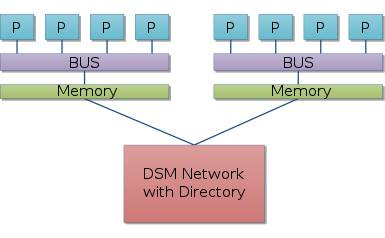
\includegraphics[width=\linewidth]{NUMA.jpg}
  \caption{schéma simplifié d'une architecture NUMA}
  \label{fig:NUMA1}
\end{figure}

Les architectures NUMA ont commencé à être étudiées, produites et vendues comme des réponses au problème
du memory gap évoqué plus haut. Pour rappel, le memory gap désigne l'écart croissant entre les performances
de calcul et les performances de bande-passante mémoire des architectures, les dernières étant désormais 
largement dépassées par les premières. Dans le cas d'une architecture disposant de très nombreux coeurs,
l'accès à la mémoire peut très vite devenir problématique dans la mesure où chacun des coeurs partagent
les mêmes ressources pour récupérer leurs données. Ainsi, si beaucoup de coeurs essaient d'accéder en
même temps à la mémoire, le temps d'accès par coeur se trouvera très dégradé, au point que l'augmentation
du nombre de coeurs deviendra contre-productive. 
\\Ce problème peut être mitigé avec les architectures NUMA. En séparant la mémoire en différents noeuds,
on essaie de diminuer les cas où plusieurs coeurs entreront en concurrence pour la même ressource. Dans
le cas idéal où chaque coeur n'accède qu'à des données situées sur son noeud, on garantit que jamais
plus de huit coeurs (si le noeud en contient huit) ne se partageront le réseau. Bien entendu, si les
coeurs commencent à beaucoup accéder à des données situées sur des noeuds distants, le problème se posera
à nouveau. Les politiques d'allocation mémoire sont conçues pour éviter au maximum ce genre de configuration.
Le système est plus flexible qu'un simple cluster dans la mesure où la communication de données entre noeuds
est transparente d'un point de vue logique - la différence ne se fait que sur le temps de transfert, là
où un système par messages, type MPI,  serait nécessaire pour un cluster. NUMA est donc un compromis 
considéré comme acceptable entre un système multicoeurs à mémoire partagée uniforme et un cluster.

\section{Avancées pendant le stage}
L'idée de base est d'observer l'interaction entre OpenMP et les architectures NUMA. Plus explicitement,
on veut savoir comment se déroule l'exécution d'un programme OpenMP sur une machine NUMA, et si 
éventuellement des comportements non-optimaux peuvent se produire, à savoir est-il possible qu'un thread
se trouve accéder à un noeud NUMA distant. Si la réponse est affirmative - et si le cas se produit 
suffisamment souvent pour être considéré comme pathologique - peut-on améliorer la situation ?
\\OpenMP ne gère jamais l'allocation des données en mémoire. De fait, les programmes reposent sur 
l'implémentation présente en local de fonctions comme malloc ou calloc, ou même à plus bas niveau
d'appels systèmes comme mmap. Une partie de mon travail a consisté à décrypter les interactions
entre chacun de ces composants : quand un programme s'éxécutant sur un cpu donné alloue une variable,
à quel moment et dans quelle partie de la mémoire elle sera réellement enregistrée ? Il m'a également fallu
décrypter le fonctionnement du support d'exécution OpenMP et notamment sa tactique quant à la migration de
tâches (un problème que nous allons expliquer ensuite). Enfin, une partie importante était de réaliser des 
benchmarks pour évaluer les pertes éventuelles dues à des accès à une mémoire distante. 
\\J'ai eu accès, dans le cadre de mes travaux, à une architecture NUMA appartenant à l'université de 
Grenoble. Cette machine, appelée Idchire, dispose de 192 coeurs répartis sur 24 noeuds NUMA distincts. 
C'est sur cette machine que j'ai réalisé les expériences que je décris dans cette partie.

\subsection{Politique d'accès mémoire sur une machine NUMA}

Comme nous l'avons dit, l'allocation des données en mémoire est indépendante du support d'exécution OpenMP.
Néanmoins, une connaissance claire de cette politique, de l'endroit et du moment où une donnée sera écrite
en mémoire est nécessaire si l'on veut appréhender comment les mécanisme d'OpenMP vont interagir avec ce
problème. Pour profiter de l'architecture NUMA, l'implémentation d'une politique spécifique est bien 
entendu requise : il faut maximiser la localité des données et faire en sorte que les accès locaux soient
la norme plutôt que l'exception. 
\\Commençons par faire un rappel sur le système de mémoire virtuelle des systèmes d'exploitations modernes.
Les premiers ordinateurs laissaient leurs programmes accéder directement à la mémoire physique de leur
système. Cela posaient de nombreux problèmes, le plus important étant celui de l'isolation des processus.
Ainsi, un programme avait la possibilité de modifier les données d'un programme voisin. Ceci représentait
une faille de sécurité majeure, dans la mesure où des programmes importants pouvaient se trouver invalidés
par le travail d'un processus annexes. Une attention toute particulière devait être accordée aux accès 
à la mémoire.
\\Pour remédier à ce problème, les informaticiens ont inventé dans les années 1960 le principe de la 
mémoire virtuelle. La mémoire physique est divisée en ``blocs'' d'une taille donnée qu'on appelle
des pages. Lorsqu'il souhaite obtenir de la mémoire, un processus va en faire la demande au système
d'exploitation, par le biais d'un appel système comme mmap. Dans l'hypothèse où il possède la mémoire 
disponible, celui-ci va alors lui attribuer un nombre de pages contenant la quantité de mémoire 
demandée. Un autre processus ne pourra, sauf appel à un mécanisme spécifique de partage de mémoire, 
accéder aux données stockées dans ces pages, réglant ainsi la question de l'isolation mémoire. Le 
système de mémoire virtuelle présente d'autres avantages, dont celui de pouvoir utiliser la mémoire 
de masse (comme un disque dur) comme extension de la mémoire vive par un mécanisme de swap : dans 
la situation où plus de pages sont attribuées qu'il n'y a de place disponible en mémoire vive, les 
pages surnuméraires sont déplacées vers le disque dur, puis rapatriées lorsque les programmes veulent
y accéder. Dans la mesure où l'accès au disque dur est plus lent que l'accès à la mémoire principale,
ce mécanisme a un impact fort sur la performance.
\\Pour pouvoir associer une adresse virtuelle et une adresse physique, on maintient une table des 
pages qui retient donc l'emplacement d'une page donnée en mémoire physique ainsi que l'identité
du processus propriétaire de chacune des pages. C'est le rôle de la MMU (Memory Management Unit),
une des composantes de l'architecture matérielle. La table des pages est stockée en mémoire, mais
une partie est maintenue dans un cache spécifique appelé le TLB (Translation Lookaside Buffer).
\\Le système de pages pose la question du choix de la taille de page appropriée. Une page trop petite
oblige les processus à faire très souvent appel au système d'exploitation et donc à déclencher un
``context switch'', ce qui est coûteux en terme de performance. D'un autre côté, une page trop large
va entraîner une forte fragmentation de la mémoire, dans la mesure où beaucoup de processus 
n'utiliseront qu'une petite fraction de l'espace qui leur aura été attribué. Le choix de la taille
de pages est donc le résultat d'un compromis entre ces deux facteurs. Aujourd'hui, une page est 
typiquement constituée de 4 Kibioctets par défaut. Cependant, la plupart des architectures propose
la possibilité d'utiliser des pages plus grandes, parfois de plusieurs mebioctets ou même d'un ou
plusieurs gibioctets. Cette option est désignée par le terme ``huge pages''\cite{hugePagesDoc}.
\\Revenons aux architectures NUMA. Dans une architecture uniforme classique, l'emplacement d'une
page en mémoire ne fait pas de différence dans la mesure où l'accès à la mémoire est partout identique.
Comme on l'a déjà expliqué, il n'en va pas ainsi pour une architecture NUMA où l'accès local est plus
rapide. La politique de choix de l'emplacement de la page est gérée par l'appel système et dépend
donc de l'implémentation de celui-ci, qui va bien entendu varier selon les systèmes d'exploitation.
Cependant, le principe général est le suivant : les pages sont allouées selon une politique ``paresseuse''
dite ``first touch''. Une allocation mémoire n'est pas faite au moment de l'allocation proprement dite
(c'est-à-dire de l'appel à malloc) mais seulement au moment où cette donnée sera accédée pour la première
fois. On délaie ainsi au maximum le travail proprement dit d'allocation. Cela permet aussi, dans 
l'hypothèse où le programmeur aurait alloué plus d'espace qu'il n'en utilise réellement, de ne payer que
pour les données réellements accédées. Dans le cas d'une machine NUMA, on apporte la garantie supplémentaire
que la page demandée sera allouée sur le noeud du processeur qui a réalisé le premier accès à la variable.
On espère ainsi faire en sorte que les données soient allouées sur les noeuds où elles seront le plus
souvent accédés.\cite{numaaware}
\\J'ai cherché à vérifier ce qu'il en était sur la machine que j'avais à disposition. Il existe une fonction
bas niveau permettant, selon les paramètres, de déplacer une page vers un noeud donné, ou encore d'obtenir 
le noeud sur lequel cette page se trouve au moment de l'appel : il s'agit de move\_pages. Ainsi l'appel
suivant :

\begin{lstlisting}
#include <stdio.h>
#include <stdlib.h>
#include <numaif.h>
#include <unistd.h>
#include <hwloc.h>

int main()
{
	int *ptr;
	intptr_t  ptr_align;

	// get page size in bytes
	int psize = getpagesize();
	ptr = malloc(25*sizeof(int));
	*ptr = 4;
	// align pointer on page boundaries
	ptr_align = (intptr_t)ptr & ~(psize - 1);
	// move_page returns 0 in case of success
	// and set status to the node number where 
	// ptr is located when fourth argument
	// is NULL
	if ( move_pages(0, 1, (void **)&ptr_align, NULL, status, 0) == 0)
		printf("memory is at node %d\n", status[0]);
	return 0;
}

\end{lstlisting}

Ce programme permet donc de connaître le noeud sur lequel se situent nos données. J'ai utilisé une bibliothèque
développé par l'Inria appelée hwloc (pour hardware locality) qui offre de nombreuses abstractions pour 
travailler à bas niveau sur des questions d'architectures (on peut ainsi récupérer des informations sur 
la machine sur laquelle le programme est exécuté, ou encore déplacer des threads ou des processus d'un coeur
à un autre). Elle m'a servi à imposer à mon programme de s'exécuter sur le CPU 0, situé logiquement sur le
noeud 0. Voici donc le programme que j'ai exécuté :

\begin{lstlisting}
#include <stdio.h>
#include <stdlib.h>
#include <numaif.h>
#include <unistd.h>
#include <hwloc.h>

int main()
{
	int *ptr;
	intptr_t  ptr_align;

	hwloc_topology_t topology;
	hwloc_cpuset_t  set1;

	//initiating locality informations
	hwloc_topology_init(&topology);
	hwloc_topology_load(topology);
	
	
	//setting process on cpu 0 with hwloc
	set1 = (hwloc_cpuset_t) hwloc_bitmap_alloc();
	hwloc_bitmap_set(set1, 0);
	hwloc_set_cpubind(topology, (hwloc_const_cpuset_t)set1, HWLOC_CPUBIND_PROCESS);


	// get page size in bytes
	int psize = getpagesize();
	ptr = malloc(25*sizeof(int));
	*ptr = 4;
	// align pointer on page boundaries
	ptr_align = (intptr_t)ptr & ~(psize - 1);
	// move_page returns 0 in case of success
	// and set status to the node number where 
	// ptr is located when fourth argument
	// is NULL
	if ( move_pages(0, 1, (void **)&ptr_align, NULL, status, 0) == 0)
		printf("memory is at node %d\n", status[0]);
	return 0;
}

\end{lstlisting}
En exécutant ce programme, j'ai eu la surprise de voir que le noeud indiqué n'était pas
nécessairement, et même rarement, le noeud 0. Le noeud semblait plutôt être
choisi aléatoirement. Je me suis d'abord demandé si la politique de first touch était 
effectivement implémentée ici. Cependant, après discussion avec d'autres membres de l'équipe,
j'ai fini par trouver l'explication. En fait, l'implémentation de malloc, avant de demander
l'allocation d'une nouvelle page, cherche logiquement à savoir si le processus ne dispose
pas déjà de la place nécessaire. Dans cette situation, une page a déjà été allouée au processus
au moment où il a été lancé, et comme elle dispose de suffisamment d'espace libre, c'est sur elle
que l'on a alloué le tableau d'entier ptr. Il faut donc faire un malloc d'un tableau suffisamment
grand pour pouvoir dépasser la capacité de la première page. C'est ce que je fais dans la version
suivante : 

\begin{lstlisting}
#include <stdio.h>
#include <stdlib.h>
#include <numaif.h>
#include <unistd.h>
#include <hwloc.h>

int main()
{
	int *ptr, * ptr2;
	intptr_t  ptr_align;
	intptr_t  ptr_align2;

	hwloc_topology_t topology;
	hwloc_cpuset_t  set1;

	//initiating locality informations
	hwloc_topology_init(&topology);
	hwloc_topology_load(topology);
	
	
	//setting process on cpu 0 with hwloc
	set1 = (hwloc_cpuset_t) hwloc_bitmap_alloc();
	hwloc_bitmap_set(set1, 0);
	hwloc_set_cpubind(topology, (hwloc_const_cpuset_t)set1, HWLOC_CPUBIND_PROCESS);


	// get page size in bytes
	int psize = getpagesize();
	// alloc first pointer and make an acces
	ptr = malloc(25*sizeof(int));
	*ptr = 4;
	// alloc second pointer and make an acces
	ptr2 = malloc(2000*sizeof(int));
	*ptr2 = 12;
	// align pointer on page boundaries
	ptr_align = (intptr_t)ptr & ~(psize - 1);
	ptr_align2 = (intptr_t)ptr2 & ~(psize - 1);
	// move_page returns 0 in case of success
	// and set status to the node number where 
	// ptr is located when fourth argument
	// is NULL
	if ( move_pages(0, 1, (void **)&ptr_align, NULL, status, 0) == 0)
		printf("memory is at node %d\n", status[0]);
	if ( move_pages(0, 1, (void **)&ptr_align2, NULL, status, 0) == 0)
		printf("memory is at node %d\n", status[0]);
	return 0;
}

\end{lstlisting}

Cette fois, si le premier tableau pointe bien un emplacement situé sur un noeud aléatoire,
le deuxième pointe bien une page située sur le noeud 0, celui qu'on attendait. On a donc
bien confirmé la politique d'allocation attendue.
\\La conséquence immédiate de ces observations est qu'un accès à des données distantes ne peut
se produire que dans le cas où un travail commencé sur un coeur donné se poursuivrait sur un autre.
On va voir dans la suite que ce cas peut se produire avec un programme OpenMP dans certaines
situations.

\subsection{OpenMP et localité des données}
On va s'intéresser ici à la manière dont un programme OpenMP va gérer la question de la localité
d'un programme - sur quel coeur ce programme va s'exécuter, est-il susceptible de migrer d'un coeur
vers un autre. On se heurte ici à une difficulté déjà évoquée auparavant : les détails de 
fonctionnement de ce genre n'étant pas mentionnés dans la spécification, ils sont spécifiques à 
chaque implémentation. Il nous faut donc maintenant choisir une implémentation particulière 
de OpenMP pour pouvoir avancer plus loin dans l'étude. On s'intéresse ici plutôt à des propriétés
de l'exécution et donc du support d'exécution OpenMP. Plusieurs choix sont possibles : le plus
classique étant l'implémentation de GCC. Autre possibilité : le support développé en open-source 
par Intel, qui a été choisi par les développeurs de Clang (le compilateur open-source lancé par
Apple) comme son support d'exécution officiel. On pourrait aussi prendre l'un des supports 
d'exécution développés par l'Inria, Kaapi et StarPU. Kaapi est tout particulièrement intéressant
dans la mesure où des membres de Corse travaillent à plein temps dessus. D'autres supports existent,
mais ils sont a priori moins intéressants.
\\Après réflexion et consultation d'autres membres de l'équipe, mon choix s'est finalement porté
sur le support d'exécution de Clang/Intel. Les facteurs décisifs ont été que ce code était 
apparemment plus facile d'entrée notamment que celui de GCC, ou que celui de Kaapi qui n'est 
pas encore suffisamment documenté. De plus, le fait que ce runtime soit d'utilisation répandue
rend plus facile de trouver de l'aide ou des renseignements sur internet. Ce choix ne nous interdit
pas d'aller regarder le fonctionnement d'autres runtime quand ils ont été spécifiquement conçus pour
les cas qui nous préoccupent.
\\Commençons par préciser la définition des termes que l'on va utiliser. En informatique, un thread
est une séquence d'instructions. Il s'agit de la plus petite séquence d'instruction qui peut être
géré de manière indépendante par un ordonnanceur. Il s'agit d'un concept proche de celui de 
processus, à une différence près : un processus possède un espace propre en mémoire virtuelle, ce
qui implique que deux processus ne peuvent interagir que par le biais d'un passage de messages.
Au contraire, un thread partage avec d'autres threads une même portion de mémoire virtuelle, ce 
qui rend possible pour deux threads de modifier la même variable. Par ailleurs, il faut distinguer
ce concept de multithreading de celui de multithreading hardware, qui est lié mais néanmoins
distinct : en termes d'architecture, le multithreading désigne la capacité d'une unité de calcul
(Central Processing Unit) à exécuter simultanément plusieurs threads logiques. Toujours en termes
d'architecture, il n'existe pas de consensus absolu pour différencier les concepts de CPU,
processeurs ou coeurs, autant de termes dont la signification peut varier selon les constructeurs
ou le contexte. On parlera surtout ici de noeud (pour les noeuds NUMA déjà évoqués au-dessus) 
ainsi que de coeur, dans le sens ``unité de calcul élémentaire'', en gardant à l'esprit que 
plusieurs coeurs peuvent partager des ressources comme des caches à différents niveaux. On se 
contentera, lorsque ce sera pertinent, de préciser quelles ressources sont partagées entre
quels coeurs, sans plus se soucier de la terminologie exacte.
\\Revenons à OpenMP et à son support d'exécution. Ce dernier se charge de créer un nombre de 
threads logiques qui lui semble approprié avant de leur répartir le travail, d'une façon que
l'on va discuter plus tard. Une remarque d'abord : le système d'exploitation a toujours la 
main sur l'ordonnancement des threads. C'est bien entendu son rôle de répartir au mieux les
ressources entre chacun des programmes essayant de s'éxécuter. Il peut donc à loisir arrêter,
redémarrer ou déplacer à tout moment n'importe quel thread en exécution. Cela peut potentiellement
poser problème même si, en pratique, les politiques d'ordonnancement sur NUMA semble éviter les 
déplacements dispensables de threads pour profiter au mieux de la localité. Cependant, les systèmes
d'exploitations, et notamment linux, offrent des outils qui permettent d'imposer à un thread logique
de rester sur un certain emplacement physique : il s'agit de la fonction pthread\_setaffinity\_np. Le
np signifie ``non-portable'' car la fonction n'est pas POSIX, mais seulement spécifique à linux.

\begin{lstlisting}[label={lst:setaff}]
#define _GNU_SOURCE

#include <pthread.h>
#include <stdio.h>
#include <stdlib.h>

int main()
{
  cpu_set_t cpuset;
  CPU_ZERO(&cpuset);
  CPU_SET(0, &cpuset);
  if (pthread_setaffinity_np(pthread_self(), sizeof(cpu_set_t), &cpuset) == 0)
    printf("successfully pinned current thread on cpu 0\n");
  return 0;
}
\end{lstlisting}
Le code présenté dans \ref{lst:setaff} donne un exemple basique de son utilisation et se contente de
déplacer et de fixer le thread courant vers le coeur 0.
\\OpenMP offre aux utilisateurs une option pour profiter de ce mécanisme. En définissant la variable
d'environnement CPU\_PROC\_BIND à true avant de lancer un programme OpenMP, on demande au runtime de 
garantir qu'un thread ne sera pas déplacé tout au long de l'exécution du programme. On met ainsi une
sécurité quant à la possibilité qu'un thread puisse être déplacé et donc avoir à accéder à des données
qu'il avait allouées sur un autre noeud. Il y a même mieux : la spécification OpenMP définit une autre
variable d'environnement, OMP\_PLACES, qui permet de fixer les threads sur des coeurs précis\cite{ompaff}. 
Ainsi, OMP\_PLACES=\{0;4\} ./example forcera le programme OpenMP example à s'exécuter exclusivement sur les
coeurs 0 à 4 (exclu). Cette option, déjà présente sur les supports d'exécution de GCC et d'Intel,
est devenu une part intégrante de la spécification depuis la version 4.0.  On voit ainsi qu'un utilisateur
avisé a la possibilité de guider le runtime pour obtenir un comportement plus optimal que ce que serait
le comportement par défaut\cite{threadaff}. 
\\Ce n'est cependant pas tout à fait le seul problème. Il faut maintenant parler de la manière dont
OpenMP répartit les tâches sur les différents coeurs. À partir de maintenant, sauf indication 
contraire, le comportement que je vais expliquer est valable pour le runtime développé par Intel, quand
bien même les autres runtimes ont généralement des stratégies similaires. Le runtime fait une distinction
entre les threads (l'unité logique d'exécution déjà définie) et les tâches (le travail - donc la suite
d'instructions - qui doit effectivement être réalisé). Les threads jouent, en quelque sorte, le rôle
de support sur lesquels les tâches s'exécuteront. Cependant, on ne peut savoir a priori sur quel thread
et donc sur quel coeur les tâches seront exécutées.
\\Décrivons un peu mieux ce fonctionnement. On a déjà décrit le processus d'outlining qui permet au
runtime de récupérer le code à paralléliser isolé par le compilateur. Ces fonctions outlinées 
représentent les tâches qui devront être exécutées par les différents threads. Au moment du premier
appel au runtime, le premier thread va créer plusieurs autres threads et éventuellement les placer
sur différents coeurs si cela a été demandé. Chaque thread maintient une file de tâche qu'il va
exécuter au fur et à mesure. La file est initialement vide pour tout le monde. Le premier thread
(le thread master) va remplir sa propre file avec les tâches qui ont été isolées par le compilateur.
Le mécanisme d'exécution est le suivant pour tous les threads : s'il y a une tâche dans la queue,
l'exécuter. Sinon, choisir un autre thread au hasard, regarder s'il a des tâches dans sa file et si
oui, lui en ``voler'' une. Si la file du thread choisi est vide, on en prend un autre au hasard. 
Dès le moment où on a trouvé une file de thread remplie, on la retient pour aller chercher de 
nouvelles tâches ensuite. 
\\Ce comportement est le même que le comportement par défaut sur Kaapi. S'il aurait pu sembler
plus logique, de prime abord, de privilégier le vol de tâche au thread master, dont on sait
qu'il possède toutes les tâches au départ, il a en fait le fait d'éviter un trop grand 
nombre d'accès concurrent à une même ressource globale (en l'occurrence, la file du thread
master). Ceci implique qu'on ne peut pas prévoir sur quel coeur sera exécutée une tâche 
particulière. La politique de first touch expliquée dans le chapitre précédent rend ce 
fait peu gênant quand une tâche n'accède qu'à des données qui lui sont privées et qui seront
donc allouées sur le noeud où elle s'exécute. Reste deux problèmes potentiels : premièrement,
le cas où plusieurs tâches partagent des données en commun. Dans cette configuration, si les
threads exécutant ces tâches sont situés sur des noeuds différents, on aura nécessairement
affaire à des accès distants. Le meilleur moyen de régler ce souci est de mettre à profit
les variables de placement des threads évoquées au dessus. Si le programmeur sait que son
programme contient de très nombreux accès à des variables partagées (ce qu'il est en général
préférable d'éviter) il lui suffit de demander que tous les threads soient situés sur le même
noeud. Bien sûr, cette approche a des inconvénients. En faisant ainsi, on limite de fait le
nombre de threads au nombre de coeurs présents sur un noeud dans l'optique où l'on veut rester
efficace. Plus important, cette approche suppose une connaissance préalable du programme non pas
du programmeur, mais de l'utilisateur, ce qui est bien sûr loin d'être évident et même relativement
rare. Deuxièmement, on a le cas où une tâche serait interrompue et reprise par un autre thread (c'est
notamment possible lorsqu'une tâche atteint une barrière). Dans ce cas, on peut envisager que la tâche
reprenne sur un noeud différent que celui sur laquelle elle avait commencé, et donc qu'il y aura accès 
à distance pour les données de cette tâche.
\\Pour ce dernier problème, plusieurs implémentations ont apporté des éléments de réponse. On peut
parler notamment d'un autre travail provenant de Inria Bordeaux appelé ForestGOMP \cite{forest}. Ce runtime
est spécifiquement conçu pour tirer le meilleur parti des architectures NUMA. En l'occurrence, les threads
sont rassemblés en ``bubbles'' qui correspondent à une notion de localité. Par exemple, des threads 
s'exécutant sur un même noeud seront placés dans la même ``bulle''. Les bulles peuvent être imbriquées : 
Si plusieurs threads dans une bulle partagent une ressource supplémentaire, comme un cache, ils pourront
alors être placés dans une nouvelle bulle à l'intérieur de la première.Dès lors, lorsqu'un thread se 
retrouve inactif et chercher à voler une tâche, il regardera en premier dans la bulle la plus interne,
puis dans la bulle de niveau supérieur, jusqu'à trouver un thread à qui prendre du travail. De la sorte,
on maximise les chances qu'une tâche soit volée par un thread proche physiquement du thread qui en avait
commencé l'exécution.
\\Voilà ce qu'il en est des questions de localité avec OpenMP. Dans le cas du runtime d'Intel, aucune 
stratégie spécifique n'est implémentée pour éviter les problèmes d'accès distants. Cependant, les différents
mécanismes annexes - le first touch, notamment - semblent constituer de bons garde-fous et permettent
a priori de limiter les cas pathologiques, même s'il est difficile de quantifier la probabilité de se
retrouver dans ce genre de conditions. 
\subsection{Évaluation de la pénalité d'un accès distant}
J'ai également cherché à mesurer quel perte on pouvait attendre d'un accès NUMA à distance. Pour cela, j'ai
cherché à réaliser des benchmarks mesurant le temps d'accès successifs à des données en mémoire.
\\La question s'est révélée plus compliquée que je ne l'avais anticipé et les questions qui se sont posées
étaient assez nombreuses. Dans la mesure où le travail fait ici a été réinvesti dans la partie suivante du
stage (de manière mieux construite et plus cohérente), il est plus simple que tout soit expliqué dans 
la partie suivante, qui évoque mon travail pour construire un benchmark qui évalue la bande-passante mémoire
sur une architecture donnée. 
\\On va simplement décrire ici sommairement le principe du benchmark. Un tableau de flottants double précision
est alloué et initialisé. Ensuite, un nombre déterminé de threads est créé (avec OpenMP). Chaque thread va 
rapatrier en boucle les données d'une portion de ce tableau dans ses registres. On mesure le temps mis par
chaque thread pour effectuer l'opération, et on en déduit une vitesse de load. En fixant les threads sur les
coeurs qu'on veut, on peut comparer les débits atteints selon que les coeurs rapatrient des données depuis leur
noeud ou depuis un noeud distant. Les détails techniques de l'implémentation seront discutés dans la partie 
suivante. Il suffit simplement de savoir que, au vu de résultats qui se sont a posteriori révélés être moins 
pertinents que je ne l'imaginais, les écarts de performances semblaient mieux s'expliquer par des effets
liés au cache et à son partage qu'à des accès distants à la mémoire.
\section{Évolution du sujet}

On avait donc affaire à plusieurs problèmes : d'abord, les seules questions soulevées par l'écriture d'un
benchmark servant à évaluer la bande-passante mémoire méritait à elles-seules une attention particulière.
Ensuite, la question de l'intérêt du travail en lui-même s'est posé : des solutions avaient déjà été 
conçues pour parer au problème général de l'utilisation d'OpenMP sur une architecture NUMA, quand bien
même ces solutions n'étaient pas implémentées sur le runtime d'Intel. À propos de ce support d'exécution,
l'appropriation du code et de son fonctionnement s'est avérée plus longue et plus fastidieuse que prévu.
En effet, le code, relativement volumineux (plusieurs centaines de milliers de lignes, ce qui n'est pas
forcément énorme comparé à d'autres projets mais reste assez peu accessible) est relativement peu documenté,
dans le sens où il manque, de l'aveu même des développeurs sur le forum dédié, une description du 
fonctionnement globale du programme. De ce fait, la simple compréhension et description du fonctionnement
a déjà pris un certain temps et l'idée d'ajouter des fonctionnalités au code devenait plus compliquée à
envisager. La question de l'intérêt proprement dit des améliorations que l'on souhaitait apporter se posait
aussi, dans la mesure où le cas paraissait trop particulier et sans doute trop rare pour pouvoir justifier
les efforts d'implémentation d'une solution. De plus, les résultats des tests ne semblaient pas aller dans 
un sens justifiant la poursuite des travaux.
\\Après discussion avec mes tuteurs, nous avons donc décidé de recadrer le travail dans une direction 
sensiblement différente. Fabrice Rastello, le chef de l'équipe, s'intéressait aux phénomènes de caches
qui pouvaient se produire lorsqu'un cache était partagé entre plusieurs threads. Il s'agissait d'abord
de réaliser un benchmark, en se basant sur les travaux déjà réalisés, permettant d'évaluer les vitesses
de load atteintes par plusieurs threads se partageant un cache et accédant à des données de taille 
variable (notamment, plus ou moins grande que le cache). Dans un deuxième temps, on voulait essayer de
construire un modèle permettant d'estimer a priori les performances atteignables dans différentes 
situations de partage. C'est donc là-dessus que j'ai recentré mon travail pour le reste du stage.


\chapter{Évaluation de la bande-passante d'une architecture}

On a donc cherché à estimer par un benchmark la bande-passante d'une architecture, ou encore la vitesse
maximale à laquelle cette architecture est capable de rapatrier des données depuis la mémoire, quel que 
soit ici le niveau de mémoire auquel on se réfère, et qui peut donc être un des niveaux de cache ou
encore la mémoire principale. En plus de cela, on cherche également à voir comment peut se comporter
cette vitesse selon qu'un ou plusieurs threads cherchent ensemble à accéder à la mémoire. Nous verrons
que des effets étonnants peuvent apparaître. Commençons d'abord par réétablir comment se construit
la hierarchie mémoire d'une architecture moderne.

\section{La hierarchie mémoire}

Le fonctionnement d'un ordinateur moderne est basé sur ce qu'on appelle le modèle de Von Neumann\cite{vonNeumann}.
Dans ce modèke, un ordinateur est divisé en les quatre éléments suivants :
\begin{easylist}[checklist]
   & Entrée (Input) 
   & Unité de contrôle
   & Unité arithmétique/logique
   & Sortie (output)
  \end{easylist}
  Ces éléments sont récapitulés dans le schéma \ref{fig:neumann}
\begin{figure}
  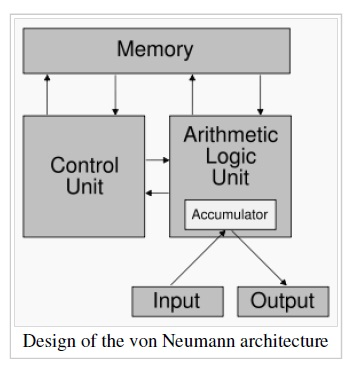
\includegraphics[scale=1]{JVN.jpg}
  \caption{schéma d'une archtecture de Von Neumann}
  \label{fig:neumann}
\end{figure}

Les noms des éléments sont assez explicites. Les entrées et sorties permettent à la machine d'interagir
avec l'extérieur : l'entrée peut être, par exemple, les signaux envoyés par un clavier ou une souris,
la sortie ceux envoyés à un écran ou une imprimante. L'unité arithmétique réalise les opérations logiques
ou arithmétiques proprement dites, comme des additions, des multiplications, des et/ou logiques. 
La mémoire sert à stocker les données et les instructions du programme. Enfin, l'unité de contrôle
s'occupe de la coordination, du séquencage des instructions et de la redirection des données et des
résultats des opérations de l'unité logique. 
\\L'opposition mémoire/unité de calcul est ici posée plus clairement. Comme on l'a déjà dit auparavant,
l'une des problématiques qui a motivé le plus de recherches et d'innovations sur les architectures dans
les dernières années est le fait que l'unité logique est aujourd'hui beaucoup plus rapide que la mémoire,
le fameux memory gap qu'on a déjà évoqué. Une des solutions déjà ancienne qui permet de pallier au souci
est que la mémoire n'est pas constituée d'un unique bloc, mais d'une stratification de niveaux croissants
en taille et en temps d'accès. C'est ce qu'on appelle la hierarchie mémoire. La mémoire la plus petite est
constitué des registres, extrêment proche physiquement des unités arithmétiques et contenant typiquement
entre quatre et jusqu'à 32  ou même 64 octets. À l'autre extrémité du spectre, on trouve la RAM 
(random-access Memory), usuellement de plusieurs Gibioctets. Dans la mesure où leur fonction habituelle 
n'est pas de stocker les données d'un programme, on ne compte généralement pas les périphériques de 
stockage type disque dur comme faisant partie de la mémoire au sens du modèle de Von Neumann, quand 
bien même cette configuration peut se produire en cas de défaut de page - le mécanisme qui permet 
d'étendre la mémoire principale en utilisant la mémoire de masse. Entre la mémoire et les registres 
se trouvent généralement des mémoires intermédiaires appelés caches. Ces caches peuvent être de nombres 
et de tailles variables. Un exemple, ainsi que des ordres de grandeur, sont présentés dans le schéma 
\ref{fig:memhier}.
\begin{figure}
  \centering
	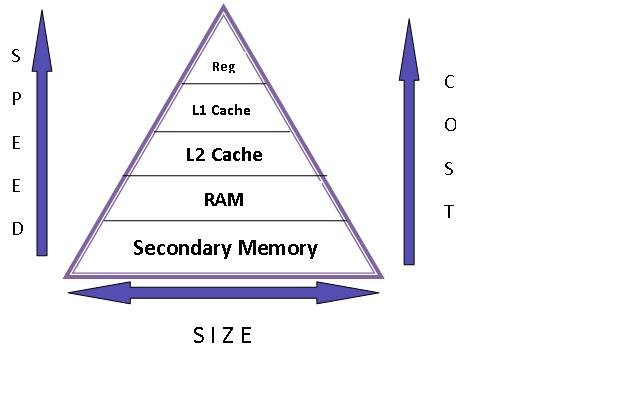
\includegraphics[scale=0.5]{hierar.jpg}
  \caption{un exemple schématique de hierarchie mémoire}
  \label{fig:memhier}
\end{figure}
\\L'intérêt de cette hierarchie est assez naturel : dans la mesure où il devenait impossible d'avoir
à la fois des mémoires assez larges pour les besoins des programmes modernes et suffisamment
rapides pour ne pas représenter un goulot d'étranglement, on a cherché un compromis en ajoutant
des mémoires intermédiaires plus petites mais plus rapides, en espérant faire en sorte que les données
les plus accédées tiendront dans un des caches. À noter que les stratégies de remplissage du cache ont
une importance cruciale, et notamment les politiques de remplacement : quelle donnée doit être 
sacrifiée et amenée vers un niveau inférieur de la hierarchie lorsqu'une autre donnée doit y être
stockée ? On aura l'occasion d'en discuter plus longuement dans la troisième partie de ce rapport.
\\Ce que nous voulons réaliser ici, c'est un benchmark qui mesure le temps d'accès aux différents 
niveaux de la mémoire, en se débarrassant autant que possible de tous les bruits pouvant perturber
la mesure.

\section{Implémentation}
Je me suis basé, pour mon implémentation, sur certains des travaux déjà réalisés par l'équipe.
Ainsi, un benchmark permettant d'estimer différents paramètres de ce type avait été codé par
mon tuteur. Il existait aussi d'autres benchmarks disponibles en ligne. J'ai notamment utilisé
un benchmark en source libre appelé STREAM. Nous allons voir d'abord le travail et les difficultés
rencontrées pour réaliser le coeur de travail, à savoir le chargement des données, puis le travail 
réalisé autour pour mesurer le temps et répartir le travail sur plusieurs threads.
\subsection{Le coeur du calcul}

Une version naïve d'un benchmark tel qu'on l'a décrit serait quelque chose de ce genre :

\begin{lstlisting}
void load(float * t, size_t siz)
{
    float res;
    for (int i = 0 ; i < size; i++)
        res = t[i]; 
}
\end{lstlisting}

Il suffirait alors de mesurer le temps d'exécution de cette fonction, puis de diviser le nombre d'octets
chargés (sizeof(float) * nombre d'itérations) par le temps obtenu.  Cette approche souffre en fait de 
plusieurs problèmes.
\\Le souci majeur ici vient de l'optimisation du compilateur. Tout compilateur moderne, à commencer
par GCC, analyse le code compilé pour repérer d'éventuelles optimisations, comme par exemple du 
code mort à éliminer ou encore des variables intermédiaires à supprimer. Le gain d'une optimisation
est difficile à estimer dans la mesure où il dépend du programme mais le temps d'exécution peut
potentiellement changer d'un ordre de grandeur. le problème dans notre exemple est que notre variable
est inutilisé, dans le sens où son élimination ne changera pas la sémantique du programme. On pourrait
simplement ajouter un print:
\begin{lstlisting}
void load(float * t, size_t siz)
{
    float res;
    for (int i = 0 ; i < size; i++)
        res = t[i]; 
    printf(``res = %d\n''); 
}
\end{lstlisting}

Mais même alors, tous les loads sont considérés comme inutiles, sauf un. Chacune des lectures réalisées
sur le tableau sera éliminée, à l'exception de la dernière. On aura donc pas le comportement attendu.
La première réaction que l'on pourrait avoir serait de désactiver l'optimisation. On aurait ainsi 
garanti que toutes les lectures seraient effectivement effectuées. Le souci que l'on aura est que dans
ce cas, des accès superflus à la mémoire seraient également réalisés, menant à un overhead considérable.
En l'occurrence, dans notre code, on ferait de la sorte chacune des lectures, mais on réaliserait 
également un accès en écriture sur la variable res à chaque itération, alors que cette variable pourrait
parfaitement être maintenue dans un registre. On ferait donc à chaque itération une lecture et une
écriture, alors qu'on voulait originalement ne réaliser qu'une lecture. Nous devons donc maintenir
une optimisation. Les développeurs de stream ne disent d'ailleurs pas autre chose :

\begin{quote}
 	3) Compile the code with optimization.  Many compilers generate
        unreasonably bad code before the optimizer tightens things up.  
      If the results are unreasonably good, on the other hand, the
        optimizer might be too smart for me!
\end{quote}

En clair : utilisez les options d'optimisation. Si les résultats sont déraisonnables, c'est que le 
compilateur a éliminé plus de code que prévu. STREAM ne fait d'ailleurs pas de benchmark sur la seule
opération de lecture : il fait des copies de tableaux ou des opérations mathématiques comme des additions
ou des multiplications.
\\Il existe plusieurs réponses possibles à cette question. La première, celle utilisée dans le benchmark
développé par mon équipe, est d'utiliser les valeurs lues dans un calcul quelconque, par exemple une 
réduction.
\begin{lstlisting}
void load(float * t, size_t siz)
{
    float red;
    for (int i = 0 ; i < size; i++)
        red += t[i]; 
    printf(``red = %d\n'', red); 
}
\end{lstlisting}
Dans cette version, on calcule la somme de tous les éléments du tableau qui est lu. Ainsi le programme
ne contient plus de code mort et l'on est sûr que chacune des lectures est réalisée. Cependant, un autre
problème se pose alors : chaque itération dépend de la complétion de l'itération précédente. C'est un souci
car les architectures modernes sont capables d'enchaîner les lectures. Une série de lectures
en mémoire est en fait généralement moins longue que le temps de lire une donnée multiplié par le nombre
de données. C'est la différence entre les notions de latence et de débit (latency et througput en 
anglais). Dans la mesure où chaque itération dépend de la précédente, on sera dans notre exemple
limité en latence et non en débit.
\\La solution est alors de dérouler la boucle et d'opérer plusieurs réductions successives. De la
sorte, on laisse le temps au programme de rapatrier plusieurs données de suite et on ne l'oblige pas
à attendre le chargement complet de la valeur suivante. Par exemple, si l'on a une latence de 5 cycles
et un débit de 2 cycles (autrement dit : charger une donnée isolée prendra 5 cycles, mais charger un grand
nombres de données seulement 2 cycles en moyenne, car le système utilise un système analogue au 
pipelining), et qu'on réalise une opération sur les données qui prend 6 cycles - les valeurs utilisées
ici sont arbitraires -, alors il faut laisser 11 cycles entre deux utilisations successives d'une 
variable de réduction. On utilisera donc 6 réductions successives, comme dans le code suivant :
\begin{lstlisting}
void load(float * t, size_t siz)
{
    float red;
    float red1;
    float red2;
    float red3;
    float red4;
    float red5;
    for (int i = 0 ; i < size; i+=6)
    {
        red += t[i]; 
        red1 += t[i+1]; 
        red2 += t[i+2]; 
        red3 += t[i+3]; 
        red4 += t[i+4]; 
        red5 += t[i+6]; 
      }
    printf(``red = %d\n'', red + red1 + red2 + red3 + red4 + red5); 
}
\end{lstlisting}
Cependant ce code présente encore des inconvénients. Le plus notable est que la latence et le débit 
sont tous deux fortement dépendants de l'architecture, mais surtout de l'endroit où réside les données
à un certain moment. On met plus longtemps, par définition, à accéder à une donnée résidant en mémoire
principale qu'à une donnée résidant dans un des niveaux de cache. De ce fait, on ne peut savoir avec
certitude quel sera la latence d'un chargement. Ceci nous oblige, de manière générale, à mettre beaucoup
de réductions, potentiellement plus que nécessaire. Cependant, insérer trop de réduction dans le code
peut faire apparaître un autre goulot d'étranglement : il peut désormais y avoir conflit pour l'accès 
aux ressources de calculs. Imaginons par exemple que dans l'exemple ci-dessus, le coeur sur 
lequel le code est exécuté ne dispose que de trois ressources d'addition de flottants. Dès lors, dans
la mesure où on essaie de faire six réductions simultanément, il y aura conflit sur chacun des éléments
de calcul et on sera potentiellement limité par le débit de ces instructions. On peut mitiger ce 
problème en utilisant plusieurs types d'opérations arithmétiques différents (par exemple des additions
et des multiplications) de sorte à maximiser le nombre d'éléments de micro-architectures utilisés.
Cependant, ceci suppose encore une connaissance pointue de l'architecture utilisée et limite 
fortement la portabilité du code. De plus, on n'est jamais complètement sûr d'être limité par
la bande-passante mémoire et pas par un autre paramètre.
\\Il existe une autre solution un peu plus directe. L'optimisation du compilateur est paramétrable,
il existe des moyens de l'éliminer partiellement ou complètement. GCC permet par exemple de désactiver
l'optimisation pour une fonction particulière. Cependant, la granularité de cette opération est encore
un peu forte pour nos besoins : on voudrait éviter absolument tous les accès mémoires superflus. Par 
exemple, même dans une simple boucle : 
\begin{lstlisting}
    for (int i = 0 ; i < size; i++)
        foo();
\end{lstlisting}
la seule incrémentation de la variable d'itération i provoque potentiellement un accès en écriture
à chaque itération de la boucle, alors que cette variable pourrait être facilement maintenue
dans un registre. Une optimisation aussi simple pourrait être effectuée même au niveau
0 du compilateur (elle l'est d'ailleurs dans l'exemple basique que j'ai rapidement compilé), 
mais on ne peut le vérifier autrement qu'en lisant systématiquement le code assembleur généré. On
est donc contraint, pour être certain que notre programme a bien le comportement désiré, d'écrire une
portion du code directement en assembleur, et de désactiver l'optimisation pour cette portion-là. On
limite ici la portabilité de deux façons : d'abord au niveau de l'architecture, puisqu'on se limite ainsi
par le jeu d'instructions qu'on va utiliser, ensuite au niveau du compilateur, puisque les options 
de désactivation des optimisations lui sont spécifiques. On se trouve donc limité, dans mon cas,
à écrire un code qui devra être compilé sur gcc et exécuté sur une architecture Intel x86-64 
(l'architecture la plus courante, et celle utilisée sur les machines sur lesquelles je faisais mes tests).
\\Cette option est celle qui a été choisie par un autre benchmark dénommé Bandwidth\cite{bandwidth} que 
j'ai découvert plus tard. Dans ce benchmark, les portions écrites en assembleur ont été rassemblées dans
des fichiers séparés et compilés à part avec le programme nasm. J'ai choisi pour ma part d'utiliser 
une option de gcc qui permet d'insérer directement de l'assembleur dans le code C. Ainsi, on évite
de rajouter une dépendance à nasm au benchmark (nasm n'était d'ailleurs pas présent sur Idchire).
\\Reste encore une question. Comme on cherche ici à saturer la bande-passante mémoire, il faudrait
pouvoir assurer qu'on charge bien au maximum les capacités du bus. Pour cela, il vaut mieux choisir
l'instruction susceptible de rapatrier le plus d'octets possibles en un seul cycle. Pour cela, on va 
utiliser non pas des instructions simples mais des instructions vectorielles. Les architectures modernes
disposent d'instructions spécifiques en mesure de travailler sur un vecteur de données et non pas sur
une donnée à la fois. Ainsi, la famille d'instructions AVX et AVX2 d'Intel permet de réaliser des 
opérations sur des vecteurs de 128, 256 ou même 512 bits pour les plus récentes. Nous utiliserons
ici des vecteurs de 256 bits. Ci-dessous se trouve le code final. L'instruction clé est vmovpapd, pour
``vectorial move double floats''
%TODO: insert codeasm.txt
Cette fonction prend en paramètre un tableau de flottant (plus précisément un pointeur), la taille de 
ce tableau et un nombre d'itérations désiré. Elle va ensuite lire le tableau linéairement autant de fois
qu'on l'aura demandé avec le deuxième paramètre.

\subsection{Autres points d'implémentation}
Nous disposons donc maintenant du coeur de travail du programme. Reste maintenant à faire tourner
ce coeur de travail et à récupérer les informations qui nous intéresse. Rappelons que l'objectif initial
de ce benchmark (et ce qui le différencie par rapport aux autres déjà évoqués) est qu'il doit pouvoir
tourner dans un contexte multi-threadé, avec un nombre de threads de préférences défini par l'utilisateur
et chargeant chacun un nombre variable de données. 
\\Il faut donc choisir une manière de créer dynamiquement le nombre demandé de threads et de leur donner
un tableau à charger. OpenMP était au départ un choix assez naturel. Il fallait trouver une manière
assez simple d'allouer des données de taille variable et de différencier le travail selon les threads.
J'ai essayé tout d'abord de réaliser l'allocation au sein de la section parallélisée, mais on rencontrait
régulièrement des erreurs au moment de l'exécution que je n'ai pas réellement réussi à expliquer. Dans
cette configuration, les mallocs échouaient dès que la taille allouée devenait trop grande. Il a donc
fallu réaliser l'allocation et l'initialisation dans la partie séquentielle. Pour cela, on récupére
le nombre de threads (qu'on indiquait en lançant le programme avec la variable 
OMP\_NUM\_THREADS) puis on alloue un tableau de taille (taille de tableau par thread *
nombre de threads) de la manière suivante : 
\begin{lstlisting}
#pragma omp parallel
	{
		nTh = omp_get_num_threads();
	}
	double arr = malloc(sizeof(double) * (sizeTab * nTh ) );
	for(int i = 0; i < nTh; i++)
	{
		for (int j = 0; j < sizeTab; j++)
			arr[i*sizeTab+j]= 3.0;
	}
\end{lstlisting}
On a pas encore distingué les tailles des tableaux ici. Ensuite, chaque thread accédait à sa portion
du tableau qui est déterminée selon son identifiant de thread, qu'on obtient grâce à la fonction
omp\_get\_thread\_num.
\begin{lstlisting}
#pragma omp parallel shared(arr)
		{
			int i = omp_get_thread_num();
			//load data from a section of sizeTab doubles of arr, do it K times
			load_asm(arr+i*sizeTab, sizeTab, K);

		}
\end{lstlisting}
De la sorte, chaque thread accède à une seule portion du tableau. K et sizeTab sont pour le moment fixé.
Reste ensuite simplement à mesurer le temps d'exécution de la fonction load\_asm. Pour cela, on utilise
une fonction mysecond basée sur l'appel clock\_gettime qui renvoie l'heure en seconde. Afin d'obtenir
un résultat plus pertinent, on réalise l'opération un certain nombre de fois (NTIMES).
\begin{lstlisting}
	for (k=0; k<NTIMES; k++)
	{
		times[k] = mysecond();
#pragma omp parallel shared( arr , timesPerTh )
		{
			int i = omp_get_thread_num();
			//load data from a section of N doubles of arr, do it K times
			load_asm(arr+i*sizeTab, sizeTab, K);
		}
		times[k] = mysecond() - times[k];
	}
\end{lstlisting}
On peut ensuite récupérer le temps minimum mesuré entre toutes ces itérations pour en déduire un débit
global. 
\\Ce n'est cependant pas tout à fait ce que l'on voulait faire au début, puisque l'on cherchait à 
avoir des threads chargeant des données de tailles différentes. On aimerait aussi pouvoir faire en sorte
qu'un thread chargeant tel tableau se trouve sur un coeur déterminé, de sorte qu'on puisse séparer les
travaux sur NUMA. Ici, OpenMP pose un problème. En effet, comme on l'a déjà évoqué, OpenMP est en mesure
de fixer des threads sur certains coeurs, mais pas de garantir qu'un travail donné pourra être réalisé
sur un coeur particulier. Comme on l'a vu dans la partie OpenMP, le travail est en effet réparti de 
manière aléatoire entre les threads. Si l'on veut fixer convenablement les threads au bon emplacement,
on se voit obligé de travailler à un plus bas niveau. D'autre part, le travail que réalise OpenMP au 
niveau du placement des threads est assez opaque et interagit de manière floue avec le reste du programme. 
Entre autres, il n'est pas évident de savoir ce qu'il adviendra d'un thread fixé préalablement sur 
un coeur qui entrerait dans une portion de code parallélisé avec OpenMP : sera-t-il ou non replacé si 
on a donné des instructions à OpenMP ? Travailler à un plus bas niveau permet d'avoir un meilleur
contrôle sur ces questions, même si cela demande plus de travail. 
\\Je me suis donc remis à utiliser la bibliothèque pthread, celle sur laquelle est basé le code 
d'OpenMP. La fonction pthread\_create prend en argument, entre autres choses, une fonction 
handler (qui contient le code que le thread va exécuter) ainsi qu'un pointeur générique permettant 
de passer des arguments. Voici la structure utilisée pour passer des arguments : 
\begin{lstlisting}
//arguments passed
//to thread handler
typedef struct 
{
	double *t;
	double * time;
	pthread_barrier_t * bar;
	long size;
	long niter;
	unsigned long *cycle;
} args_t;
\end{lstlisting}
Les pointeurs time et cycle servent à renvoyer les valeurs de temps d'exécution en secondes et en 
nombre de cycles au thread principal. La barrière permet d'attendre que le thread principal ait déplacé
chacun des threads vers leur destination avant de commencer le travail. Voici maintenant le code du 
handler proprement dit : 
\begin{lstlisting}
void * handler(void * arg)
{
	args_t * args = (args_t *) arg;
	//size of data that are to be loaded 
	//by this thread
	double ld = sizeof(double) * args->size * args->niter;
	double time;
	unsigned long cyc; 
	int cpu;


	// barrier (waiting for everyone to be pinned)
	pthread_barrier_wait(args->bar);

	cpu =  sched_getcpu();


	cyc = get_cycles();
	time = mysecond();
	load_asm(args->t, args->size, args->niter);
	time = mysecond() - time;
	cyc = get_cycles() - cyc;
	*(args->time) = time;
	*(args->cycle) = cyc;
	printf("Fast thread has taken %11.8f s to execute on cpu %d, data : %ld bytes loaded %ld times\n \
Throughput : %f %cB/s \n", time, cpu, args->size * sizeof(double),  args->niter, siz_d(ld / time), units_d(ld / time));

	return NULL;
}
\end{lstlisting}
On récupère et affiche également le numéro du coeur sur lequel le thread s'est exécuté.
\\Il suffit désormais de récupérer les tailles des tableaux qu'on veut charger et de les passer en 
paramètres dans une structure. Pour cela, on se contente de les récupérer par la sortie standard. 
Ceci permet un usage plus commode. On peut écrire les tailles des tableaux désirées dans un fichier 
et le passer par le biais d'un pipe au programme, comme ceci : 

\begin{lstlisting}[language=bash]
cat threadsizes.txt | ./load 
\end{lstlisting}

De cette manière, on a un programme qui permet d'obtenir les débits individuels de chacun des threads 
ainsi que le débit global dans le thread principal.
\\Pour le cas des architectures NUMA, on voulait disposer d'une option du programme pour différencier
un nombre donné de threads et les exiler sur un autre noeud. J'ai procédé de la manière suivante :
en premier lieu, j'ai ajouté deux options à mon code, une option ``-slow'' qui permet de préciser le
nombre de threads qu'on veut ostraciser (slow car ces threads atteindront vraisemblablement une vitesse
moins importante) et l'option ``-places'' qui permet de placer les threads slow sur un noeud différent
des threads slow. Au début du programme, le thread principal est placé sur le thread 0. Les autres 
threads sont ensuite créés, puis placés sur les coeurs appropriés. De la sorte, si le fichier 
threadsizes.txt est comme suit : 
\begin{lstlisting}[language=bash]
1000000
1000000
1000000
2000000
\end{lstlisting}

alors la commande suivante crée trois threads normaux chargeant chacun un tableau de 1000000 flottants
double précision et un thread ostracisé chargeant un tableau de 2000000 flottants double précision.
\begin{lstlisting}[language=bash]
cat threadsizes | ./load -slow=1 -places=spread
\end{lstlisting}
Par ailleurs, quelques problèmes techniques se sont posés. Ainsi, le programme se terminait de temps à 
autre sur une erreur de segmentation. Il m'a fallu un peu de recherche pour me rendre compte que 
l'instruction de load que j'utilisais réclamait un pointeur aligné sur 32 octets. Il est donc nécessaire d'aligner notre tableau, ce que je fais grâce à la fonction suivante : 
\begin{lstlisting}
//takes a pointer and returns it
//rounded up on upper n bound
char * align_ptr(char * t, intptr_t n)
{
	intptr_t ptr;
	ptr = (intptr_t)(t + n) & ~(n - 1);
	return (char *)ptr;
}
\end{lstlisting}
Par ailleurs, sur un plan plus pratique, la question du nombre d'itérations à exécuter s'est posée. Ce 
nombre était au départ statique, mais cela avait pour conséquence que le temps d'exécution du programme
variaient avec la taille du donnée, au point d'ailleurs qu'il devenait beaucoup trop long pour des 
données trop grande, par exemple pour plusieurs méga ou même gigaoctets. L'autre conséquence est 
que chaque thread aura un temps d'exécution différent, ce qui fausse la donne par rapport aux
phénomènes que l'on veut observer. Pour améliorer mon programme sur la question, j'ai choisi 
de calculer un nombre d'itérations dépendant de la taille du tableau donné en entrée. Le 
calcul est assez simple : 
\begin{lstlisting}
long get_nb_iter(long size)
{
	long k = 64;
	if(size < 64)
	{
		cout << "array too small !!" << endl;
		abort();
	}
	while(k * size * DOUBLE_PER_CYCLE < TOTAL_CYCLES )
		k = k << 1;
	return k;
}
\end{lstlisting}
TOTAL\_CYCLES est un nombre arbitraire fixé à $2^{28}$, qui représente le nombre approximatif de cycles
que l'on veut voir exécuté par chaque thread. DOUBLE\_PER\_CYCLE est fixé à 2 et représente une 
approximation (evidemment fausse) du nombre de doubles pouvant être chargé en un cycle. Dans la mesure
où ce nombre varie selon que l'on charge depuis un cache ou depuis la mémoire principale, ce calcul
est bien entendu peu précis, mais il permet au moins de faire en sorte que toutes les exécutions aient
le même temps de calcul en ordre de grandeur. 
\\Le programme ayant ainsi été écrit et testé dans la mesure du possible (vérification que les éléments
en mémoire étaient bien chargés, ou que le nombre d'itérations était bien celui attendu), il peut 
servir de base à l'analyse des architectures à disposition, ainsi que comme vérification des futures
prédictions. 

\section{Tests et résultats}
On a déjà évoqué la machine Idchire sur laquelle on faisait nos tests. Dans la mesure où cette machine
a connu des problèmes de maintenance et a été à plusieurs reprises indisponibles, mais aussi parce qu'il
était plus intéressant de disposer de plusieurs architectures, j'ai eu accès à une autre machine, gérée
celle-ci directement par l'équipe, et dénommée Dracula. Celle-ci possède quatre coeurs sur un seul noeud,
tout en étant d'une génération plus récente que Idchire et possédant donc quelques instructions 
supplémentaires. Nous allons donc voir ce qu'ont donné les tests pratiqués sur ces machines et les
conclusions qu'on a pu en tirer.
\subsection{Tests sur la machine NUMA}
Revenons d'abord sur le sujet qui a occupé la première partie de mon stage. Si, dans le dernier chapitre,
je présente une version aboutie du benchmark que j'ai construit, l'ensemble des connaissances 
nécessaire à sa réalisation, ainsi que des différents pièges et difficultés n'ont été acquises que 
progressivement. Ainsi, les premiers tests que j'ai pu effectués l'ont été avec une version très naïve
de ce qu'allait ensuite devenir le programme. Le benchmark tel que je l'avais écrit sur le moment 
était notamment compilé sans optimisation, sans que je mesure l'impact qu'une telle décision pouvait
avoir sur la performance. Le fait que les placements de threads d'OpenMP pouvait avoir une influence
sur le comportement du programme même après la sortie de la zone parallélisé m'échappait. Enfin, les
accès réalisés n'étaient pas vectoriels et on peut imaginer que je n'utilisais pas toute la 
bande-passante disponible.
\\Tous ces paramètres ont fait que la différence entre les accès distants et locaux semblaient 
négligeables : un accès distant ne paraissait pas prendre particulièrement plus de temps, du moins
en lecture. Une différence plus notable semblait se faire sur des accès en écriture, mais les temps
n'étaient pas stables non plus. Les résultats étant difficiles à interpréter, j'essayais d'en 
chercher la cause dans diverses directions, notamment dans des effets de préfetch. Certaines 
architectures modernes peuvent faire une supposition raisonnable sur les prochaines données qui
seront accédées et tenter de les rapatrier en avance dans le cache. Il paraissait sur le moment
plausible que cette stratégie puisse mitiger les écarts de performance, surtout dans la mesure où
mes accès étaient linéaires et particulièrement prévisibles. Une politique de localité qui rapatrierait
par avance les données consécutives à celles déjà accédées était susceptible dans mon cas de donner
de bons résultats. Cependant, mes recherches effectuées sur le sujet ne semblaient pas montrer
l'existence d'un préfetch hardware automatique très avancé en l'état actuel de la technologie.
Il est vrai que le secret tenu par les constructeurs comme Intel sur leurs design pouvait
éventuellement expliquer le peu de littérature sur le sujet. De fait, la technologie semble 
aujourd'hui limitée au prefetch d'instructions (le flot étant plus prévisible) ou éventuellement
au prefetch software, guidé par le programmeur \cite{prefetchgcc}.
\\J'ai eu l'occasion de revenir plus tard sur ces premiers résultats avec plus de recul et beaucoup
plus de maitrise que je n'en avais sur le moment. Avec un programme au point et bien testé, il
a finalement été possible de mettre en évidence des écarts de performances très notables. Les 
comportements ressemblent plus à ceux auxquels on pouvait s'attendre. Tant que les données chargées
d'une part par les threads locaux, d'autre part par les threads distants tiennent dans le cache 
que partagent tous les coeurs d'un même noeud, il n'y a aucune différence de performance. Cependant,
dès que les données chargées ne tiennent plus dans le cache et qu'on doit donc accéder à la mémoire
principale, et donc à un noeud distant pour les threads ostracisés, on observe la différence de 
performance attendue. Par exemple, sur Idchire qui possède un cache de 20 Mébioctets, 2 threads
chargeant chacun 96 Mebioctets, l'un depuis le noeud local, l'autre depuis le noeud distant,
atteindront respectivement des débits de 10GB/s et 2GB/s respectivement, soit une perte de plus
de 80\%. Aucune perte n'est par contre observable si les threads chargent significativement 
moins de 20 mebioctets.
\subsection{Partage des ressources}
\label{subsec:ressources}
J'ai fait tourner mon benchmark, pour différents nombres de threads (dans la limite du nombre de coeurs
partageant un cache) et avec une taille de tableau croissante. Dans un premier temps, chaque thread 
réalise exactement le même travail. Les graphiques \ref{fig:idchbench} et \ref{fig:dracbench} 
montrent l'évolution de la bande-passante globale respectivement sur Idchire et Dracula. Il est à 
noter que les threads ont un comportement très symétrique, aucun ne semble prendre le pas ou être
plus pénalisé. C'est pour cela que l'on se contente d'afficher la bande-passante globale. La taille
du cache est indiquée par la ligne verticale rouge.
\begin{figure}
  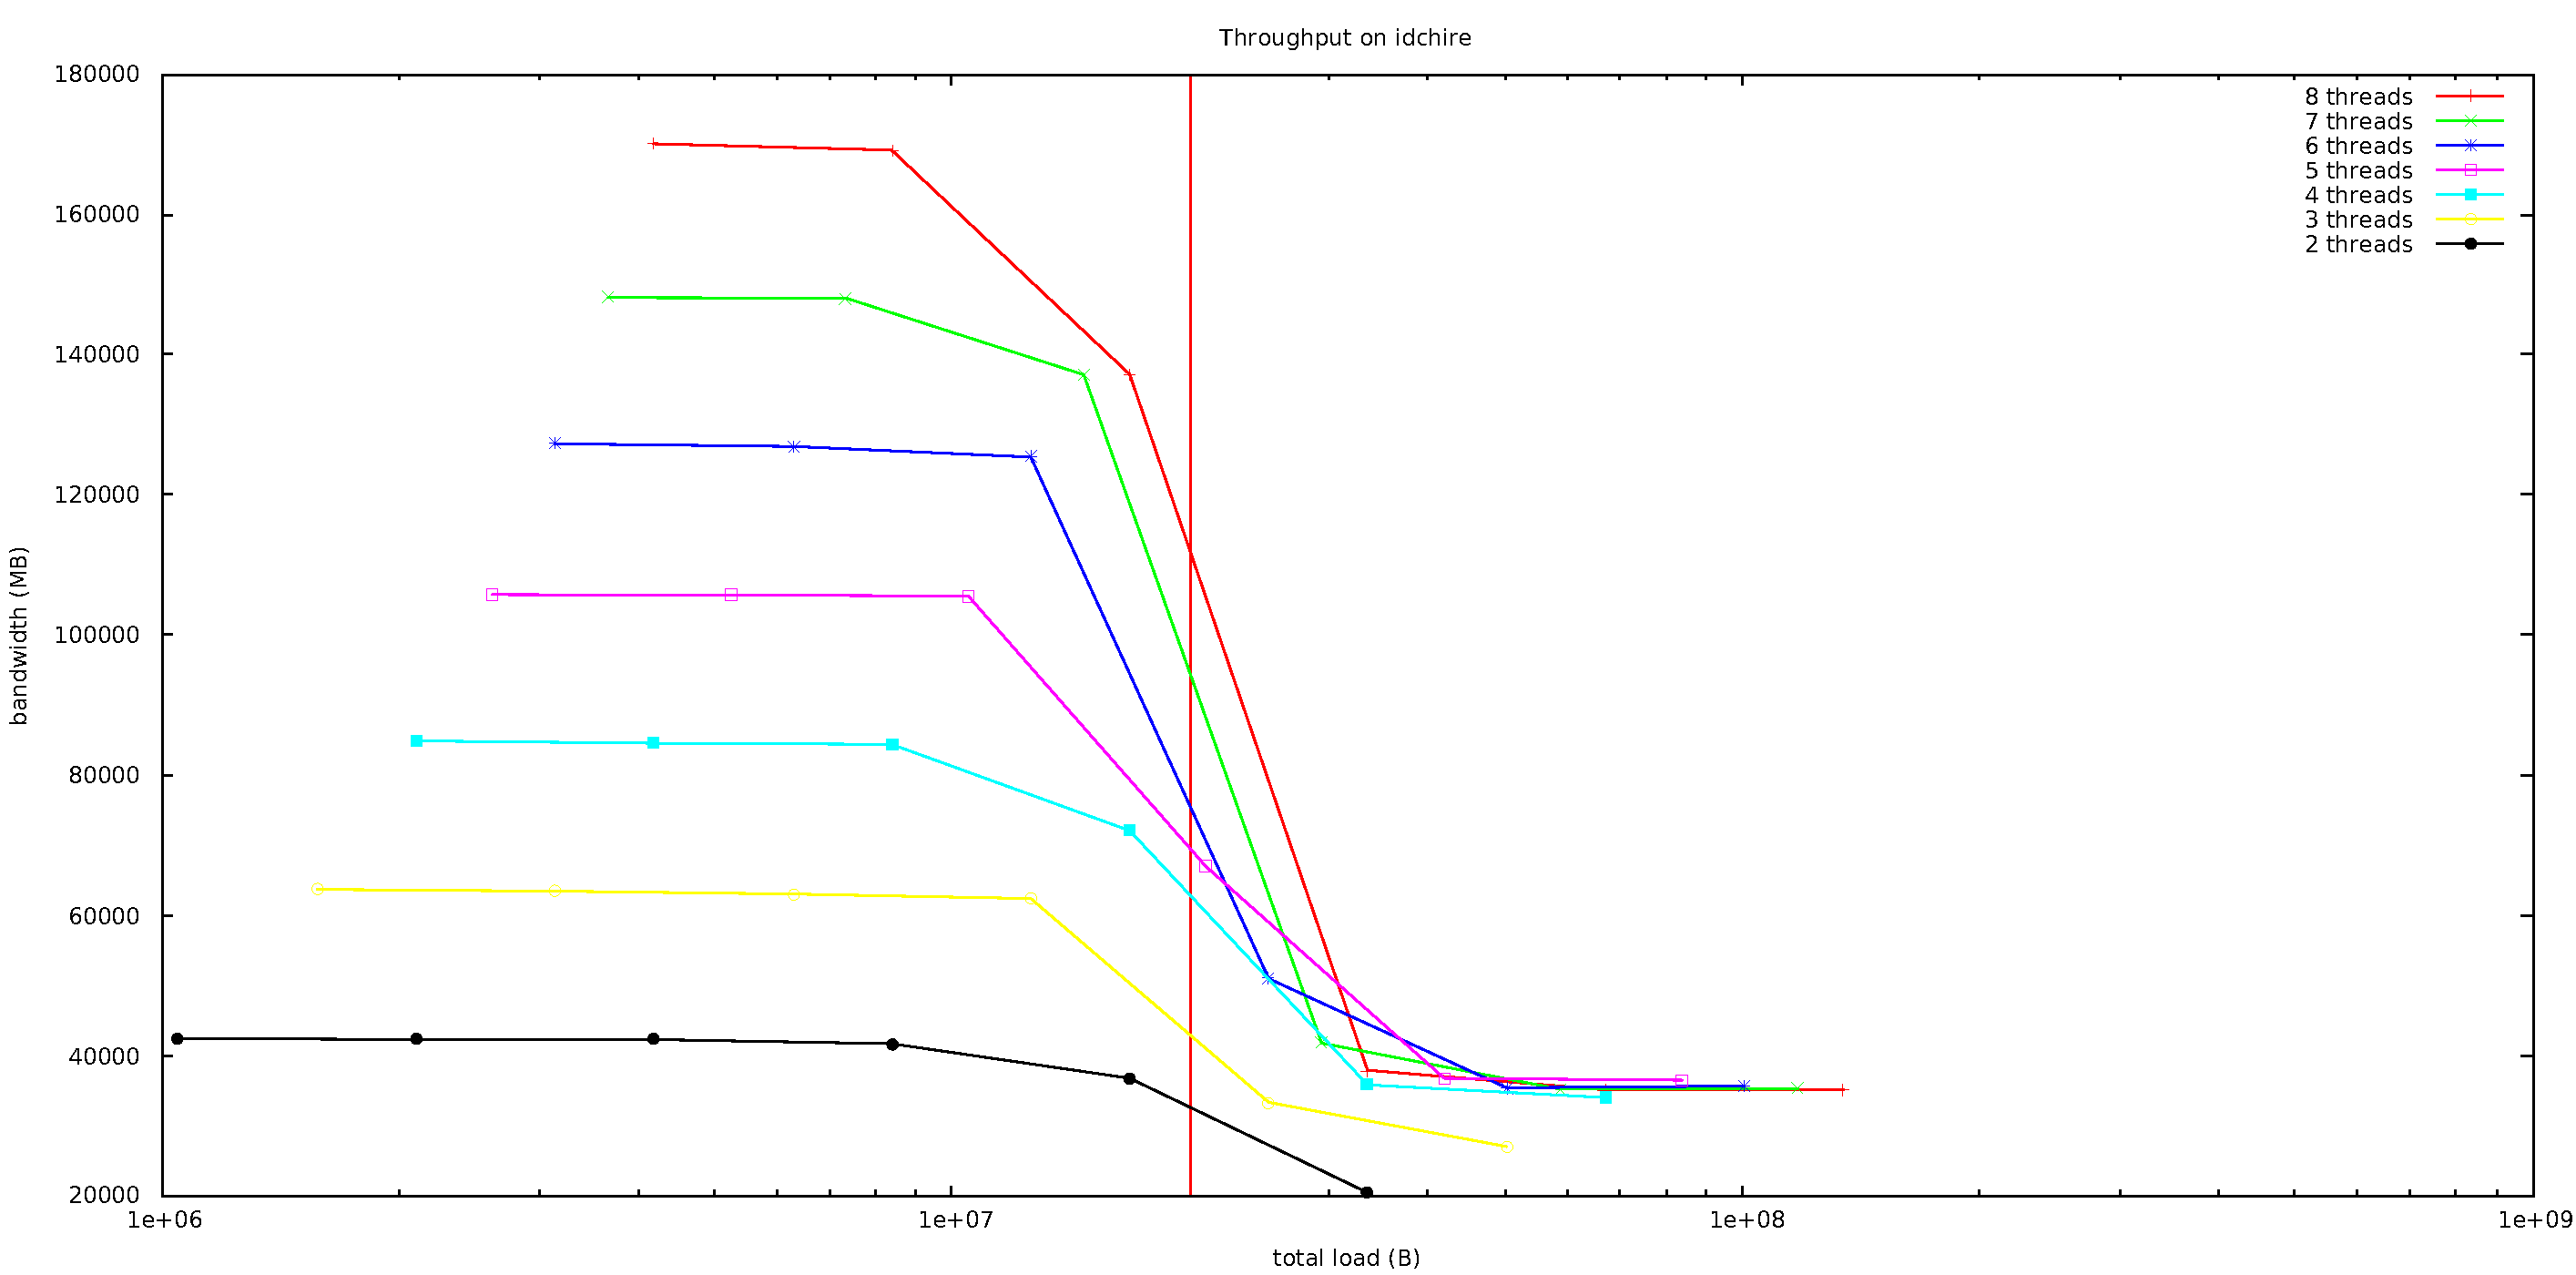
\includegraphics[width=\linewidth]{bandwidth_idch.pdf}
  \label{fig:idchbench}
\end{figure}
\begin{figure}
  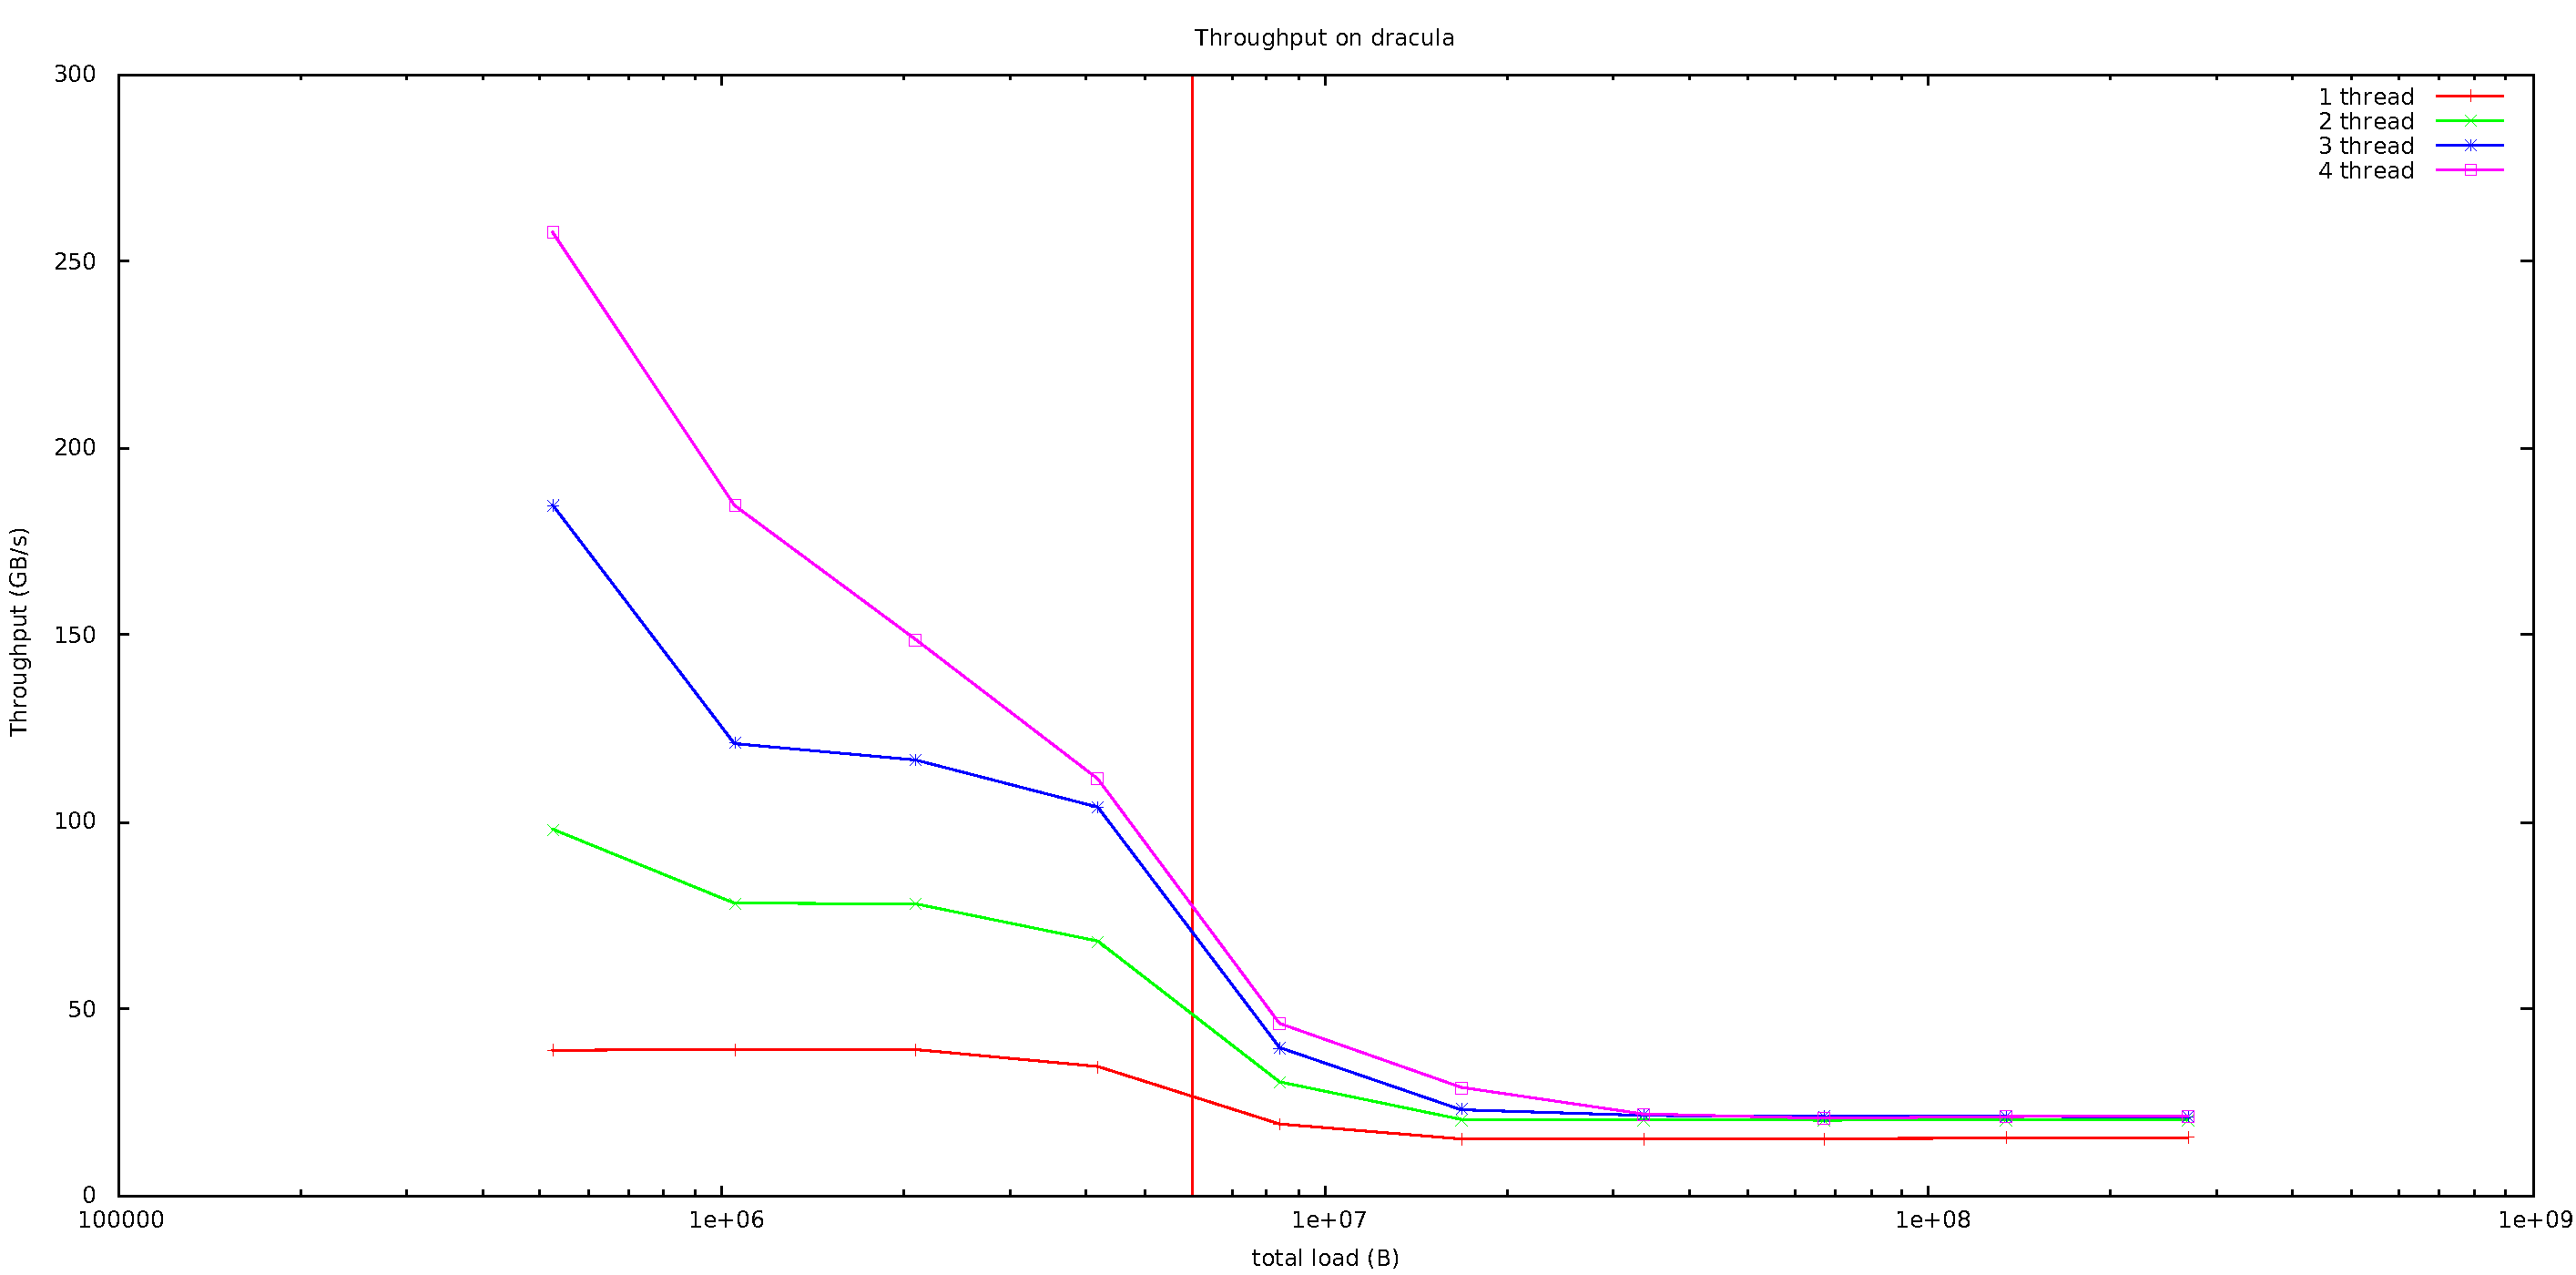
\includegraphics[width=\linewidth]{bench_dracula.pdf}
  \label{fig:dracbench}
\end{figure}
On apprend d'autres choses grâce à ces graphiques. Notamment, le partage des ressources se fait
différemment selon que les données tiennent ou non dans le cache. On s'aperçoit que le débit global est 
proportionnel au nombre de threads lorsque les données tiennent dans le cache (donc que le débit 
individuel est constant relativement au nombre de threads pour une quantité de données fixée). Ce débit
global est par contre constant lorsque les threads vont chercher leurs données en mémoire. Cela signifie
que les threads n'interfèrent pas entre eux lorsqu'ils chargent des données depuis le cache, 
mais qu'ils entrent en concurrence et se partagent la bande-passante disponible lorqu'ils doivent 
accéder à la mémoire principale.
\\Autre observation : sur chacune des deux architectures, il faut un certain nombre de threads pour
atteindre la saturation de la bande-passante. Ainsi, sur dracula, on voit que quand le seuil de
20 GB/s est atteint avec deux, trois et quatre threads, un thread seul n'arrive pas à faire
mieux que 15 GB/s. De même, sur dracula, là où cinq, six ou huit threads parviennent à obtenir
un débit global de 35GB/s environ, moins de quatre threads ne parviennent pas à saturation.
\\Ces résultats laissent supposer que plusieurs ressources sont en jeu qui peuvent chacune
faire office de goulot d'étranglement pour la bande-passante globale. La ressource partagée devient
limitante quand trop de threads essaient d'en profiter à la fois. Lorsque ce n'est pas le cas,
c'est la ressource individuelle qui devient limitante. 
\subsection{En guise de première conclusion }
Nous avons donc programmé un benchmark d'évaluation de la bande-passante mémoire qui permet 
d'estimer les capacités en mémoire. Il a la particularité d'être utilisable en multithread
comme dans un programme simple, et d'être plus modulable qu'un programme comme bandwidth, même
si ce dernier est adapté à plus d'architecture et qu'il teste plus exhaustivement les ressources.
Mon travail a été intégré dans la suite de benchmarks de l'équipe (sous l'impulsion d'un étudiant 
invité dans l'équipe qui travaille sur un projet de normalisation et de mise en commun des benchmarks 
dans le monde scientifique). Il a également été utilisé dans le cadre d'un autre projet de l'équipe
qui a besoin de diverses méthodes pour estimer les ressources d'une machine.
\\Fort de ces résultats, on peut maintenant s'attaquer au problème qui nous motivait
au départ : la prédiction des performances et du partage du cache par différents threads.

\chapter{Modèle de prédiction de bande-passante et d'accès au cache}
Ce travail a occupé toute la dernière partie de mon stage. Il est encore incomplet, quand bien
même il offre certaines promesses - ainsi que des limitations qui n'ont pas encore pu être dépassées.
Savoir s'il sera poursuivi est une autre question qui n'a pas encore de réponse - peut-être serai-je
en mesure de reprendre et d'apporter une conclusion un peu plus tard. En attendant, je vais
présenter ici l'état dans lequel je me suis trouvé à la fin du stage. Il manque encore, au minimum,
un test plus poussé de la dernière version du modèle qui nous permettrait d'évaluer sa pertinence.
On avait construit sur la fin un modèle de prédiction sur une base empirique, comme on l'expliquera
dans la suite. Nous allons néanmoins commencer par poser quelques bases sur le fonctionnement d'un
cache dans une architecture et les problématiques qui se sont posées.

\section{Cache et bande-passante}
Le principe du cache et son intérêt avait déjà été présenté plus haut dans le chapitre sur la 
hierarchie mémoire. L'idée est d'offrir aux coeurs des portions de mémoire plus proche et plus 
rapide que la mémoire principale, et d'espérer que le programme trouvera aussi souvent que possible
une donnée dans le cache et non dans la mémoire. En effet, les emplacements du cache ne sont pas
réellement adressables : toute donnée présente dans un cache est une réplication d'une donnée
présente dans la mémoire. Lorsqu'un coeur veut faire un accès à une donnée, il s'adresse à son 
cache pour savoir s'il détient cette donnée. Si c'est le cas, on a un hit et l'utilisation du
cache était gagnante. Sinon, on a un miss, le coeur doit aller chercher sa donnée en mémoire,
ce qui entraîne une pénalité. Le débit atteint par un programme va dépendre fortement du taux
de miss et du nombre de fois où il a dû aller chercehr une donnée en mémoire. Plus ce taux est
important, plus le débit est faible.
\\Une architecture peut disposer de plusieurs niveaux de cache, les niveaux étant de taille
croissante et de vitesse d'accès décroissante. Chacun des niveaux peut être partagée par plusieurs
coeurs ou être privé. En général, le tout dernier niveau est partagé, alors que les niveaux au-dessus
sont privés. Par exemple, Idchire et Dracula disposent tous deux de trois niveaux de caches, les deux
premiers étant privés tandis que le dernier est partagé entre tous les coeurs pour Dracula, et entre
tous les coeurs d'un noeud (donc entre huit coeurs) pour Idchire.
\\Le fait qu'il existe plusieurs niveaux de cache oblige à répondre à des questions sur la localité
et la duplication des données : une donnée situé dans le cache le plus proche du coeur doit-elle ou
non se trouver dans les caches en dessous ? Les constructeurs proposent différents types de réponses
à cette question que nous n'allons pas développer ici. De même, le partage d'un cache impose de 
répondre à des problématiques de maintien de la cohérence entre des données partagées que nous ne
traiterons pas non plus. Nous ne parlerons pas plus de la question du moment où une écriture
qui a été faite dans le cache sera répercutée en mémoire principale. Ce document \cite{cachebus} 
quand bien même il est déjà ancien, fait une bonne synthèse de tous ces sujets dans sa première
partie.
\\Ce qui nous intéresse surtout ici, c'est la politique de remplacement des données dans le cache. 
Quand le cache est rempli et qu'un accès quelconque à une donnée non présente dans le cache est
fait, la donnée accédée est placée dans le cache de manière à pouvoir être disponible plus 
rapidement pour un prochain accès. On tire ici parti du principe de localité temporelle qui 
veut qu'une donnée accédée récemment ait toutes les chances d'être réaccédée rapidement dans 
le futur. La question est de savoir quelle donnée sera sacrifiée pour laisser sa place à la
nouvelle arrivée. Plusieurs paramètres interviennent à ce moment-là.
\\Précisons d'abord que la granularité de base d'un cache est la taille de ce qu'on appelle
un bloc ou une ligne, une valeur courante étant 64 octets. Cela signifie que les données
sont toujours stockées dans le cache par bloc de 64 octets consécutifs, jamais moins. La
question est de savoir combien d'emplacements sont disponibles dans le cache pour un bloc
d'une adresse particulière. La réponse est le résultat d'un compromis : si une ligne pouvait
être stockée n'importe où dans le cache, alors il y aura une pénalité importante liée au coût
de la recherche de la donnée dans le cache. D'un autre côté, si une adresse ne pouvait être
stocké qu'à un seul emplacement, on pourrait s'attendre à ce que le cache soit utilisé de 
manière suboptimale. Le nombre de choix possibles pour une ligne est appelé l'associativité
du cache. Cette associativité est de 12 pour Dracula. L'ensemble d'emplacements dans lequel
une ligne peut être mise en cache est appelé un set.
\\La question est donc de savoir comment est fait, dans un set, le choix de la ligne qui sera
remplacée. À nouveau, bien des techniques existent et dépendent du constructeur. Une technique
simple à mettre en place serait d'implémenter un simple FIFO (First-In First-Out). Seulement,
cela signifierait qu'une donnée entrée dans le cache il y a un long moment, mais qui a été utilisée 
à de nombreuses reprises depuis, pourrait être évictée au profit d'une donnée entrée dans le cache 
plus récemment mais qui n'aurait pas été réutilisée depuis. Une politique plus élaborée serait
simplement de choisir le LRU (Least Recently Used) à savoir l'élément le moins récemment accédé. 
Pour des raisons d'implémentations, il existe des versions plus simples censées approximer un 
comportement de LRU dénommée PLRU pour Pseudo-LRU. On décrira cette stratégie un peu plus loin, 
avec quelques autres, quand il s'agira de les émuler. Ces bases suffiront pour le moment.
\section{Premières tentatives}
Le problème de la politique de remplacement est que son implémentation n'est pas rendu publique
par les constructeurs et notamment par Intel. Dans un premier temps, l'hypothèse a été faite
que l'architecture suivait peu ou prou une politique LRU, qui est certainement la plus répandue
dans l'ensemble des politiques de remplacement de cache (sans parler spécialement de cache 
de processeur). La question est alors la suivante : étant donné un nombre de thread et la 
quantité de données auxquelles ils vont accéder, que pourra-t-on dire des débits que chacun 
des threads pourra espérer atteindre ? Le cas qui nous intéresse réellement est celui où
la somme des données accédées par les threads est supérieure à la taille du cache, mais où
au moins certains threads accèdent à des données de taille inférieure au cache. Les prévisions
sont simples dans le cas où la totalité des données tient dans le cache (taux de miss de 0 
pour tout le monde) ou celui dans lequel aucun des threads n'a de données tenant dans le
cache (taux de miss attendu de 1).
\\L'intuition de base était la suivante : quand un thread accédait à un plus grand nombre de
données, ou encore accédait à ses données plus lentement que d'autres, alors il risquait
de voir ses données constituer une cible privilégiée pour l'éviction. De ce fait, on s'attendrait
à ce qu'il subisse un nombre de miss plus important, et donc qu'il soit pénalisé en terme de
bande-passante. Restait à formaliser cette intuition plus convenablement.
\\J'ai formulé une première prévision pratique. Toujours en supposant une politique LRU, on
peut affirmer la chose suivante : 
\newtheorem{th1}{Théorème}
\newtheorem{th2}{Théorème}
\begin{th1}
Soit N un nombre de threads, $T_1, T_2, \cdots T_N$ les tailles des données auxquelles ces threads
accèdent respectivement. Pour tout thread i, si $T_i$ est inférieur à $\frac{C}{N}$, où C est la 
taille du cache, alors le thread i ne subira aucun miss.
\end{th1}
Pour la preuve, on fait aussi l'hypothèse que, comme dans notre benchmark, l'accès aux données
est linéaire et boucle sur lui-même. C'est une hypothèse forte mais elle permet d'avoir une 
bonne idée du moment où une donnée va être réaccédée, ce qui autorise une réflexion plus formelle.
On espère simplement que les résultats obtenus pourront être au moins qualitativement pertinents
pour d'autres types d'accès. On suppose aussi que toutes les tâches ne font que des accès mémoire
(pas de travail ou de calcul annexe). 
\begin{proof}
Soit N un nombre de threads, $T_1, T_2, \cdots T_N$ les tailles des données auxquelles ces threads
accèdent respectivement. Soit C la taille du cache. On va supposer que :
$\forall i, T_{i} < T_{i+1}$
On définit ici le concept de distance de réutilisation pour une donnée. Il s'agit, pour une 
donnée d, du nombre de données qui ont été accédées par tout le monde entre deux accès successifs
à d. On va noter $\Delta(d)$ = distance de réutilisation de d, et $\delta_{i}(t)$ le nombre de 
données accédées par le thread i entre deux accès à d.
Comme on a fait l'hypothèse que le cache fonctionne en pur PLRU, alors la question est de
savoir si $\Delta(d) < C$. Si oui d se trouve dans le cache, sinon il a été évicté.
\\Soit i tel que $T_i \leq \frac{C}{N}$. Soit t une donnée accédée par i.
On a $\forall j \leq i, T_{j} \leq T_{i} \leq \frac{C}{N}$.  On peut en déduire que $\forall j < i, 
\delta_{j}(t) \geq \frac{C}{N}$.
D'autre part, si un thread accède à plus de données qu'un autre, il a plus de chance de faire
des miss et va donc au moins aussi lentement.
Donc pour $k > i$, comme ${T_{k}}\geq{T_{i}}$, on peut affirmer que $\delta_k(t)\leq \frac{C}{N}$.
\\Dès lors, on a : $\Delta(t) = \sum_{j=1}^{N} {\delta_{j}(t)} \leq \sum_{j=1}^{i-1}{\frac{C}{N}} + 
T_i + \sum_{k=i+1}^{N}{\frac{C}{N}} \leq N * \frac{C}{N} $.
\\Donc $\Delta(t) \leq C$. On a prouvé que le thread i trouve toujours ses données dans le cache.
\end{proof}
On sait que l'hypothèse de LRU est forte ne serait-ce que parce que le cache n'est pas totalement
associatif. Néanmoins, si on suppose une politique LRU à l'intérieur d'un set, alors on peut 
légitimement supposer qu'un comportement similaire sera adopté sur l'ensemble des données si 
les sets sont remplis uniformément.
\\J'ai cherché à vérifier expérimentalement cette règle. Pour cela, j'ai fait tourner mon
programme sur idchire avec les paramètres suivants : un thread chargeant des données de plus
en plus large fait des lectures. On fait tourner en parallèle un autre thread qui charge lui 
des données beaucoup plus grande (plusieurs fois la taille du cache) puis deux autres, puis 
trois, etc. et on regarde les performances du premier thread. Les résultats sur Dracula
et Idchire sont présentés en figure \ref{fig:dracasbench} et \ref{fig:idchasbench}. 
\\La loi n'est pas parfaitement suivie, notamment sur Dracula, mais on voit néanmoins qu'elle
décrit correctement le comportement des threads au moins d'un point de vue qualitatif. Cependant,
elle n'est pas très satisfaisante parce qu'elle ne décrit qu'un cas particulier. On aimerait
pouvoir intégrer des situations plus générales dans le modèle.
\begin{figure}[H]
  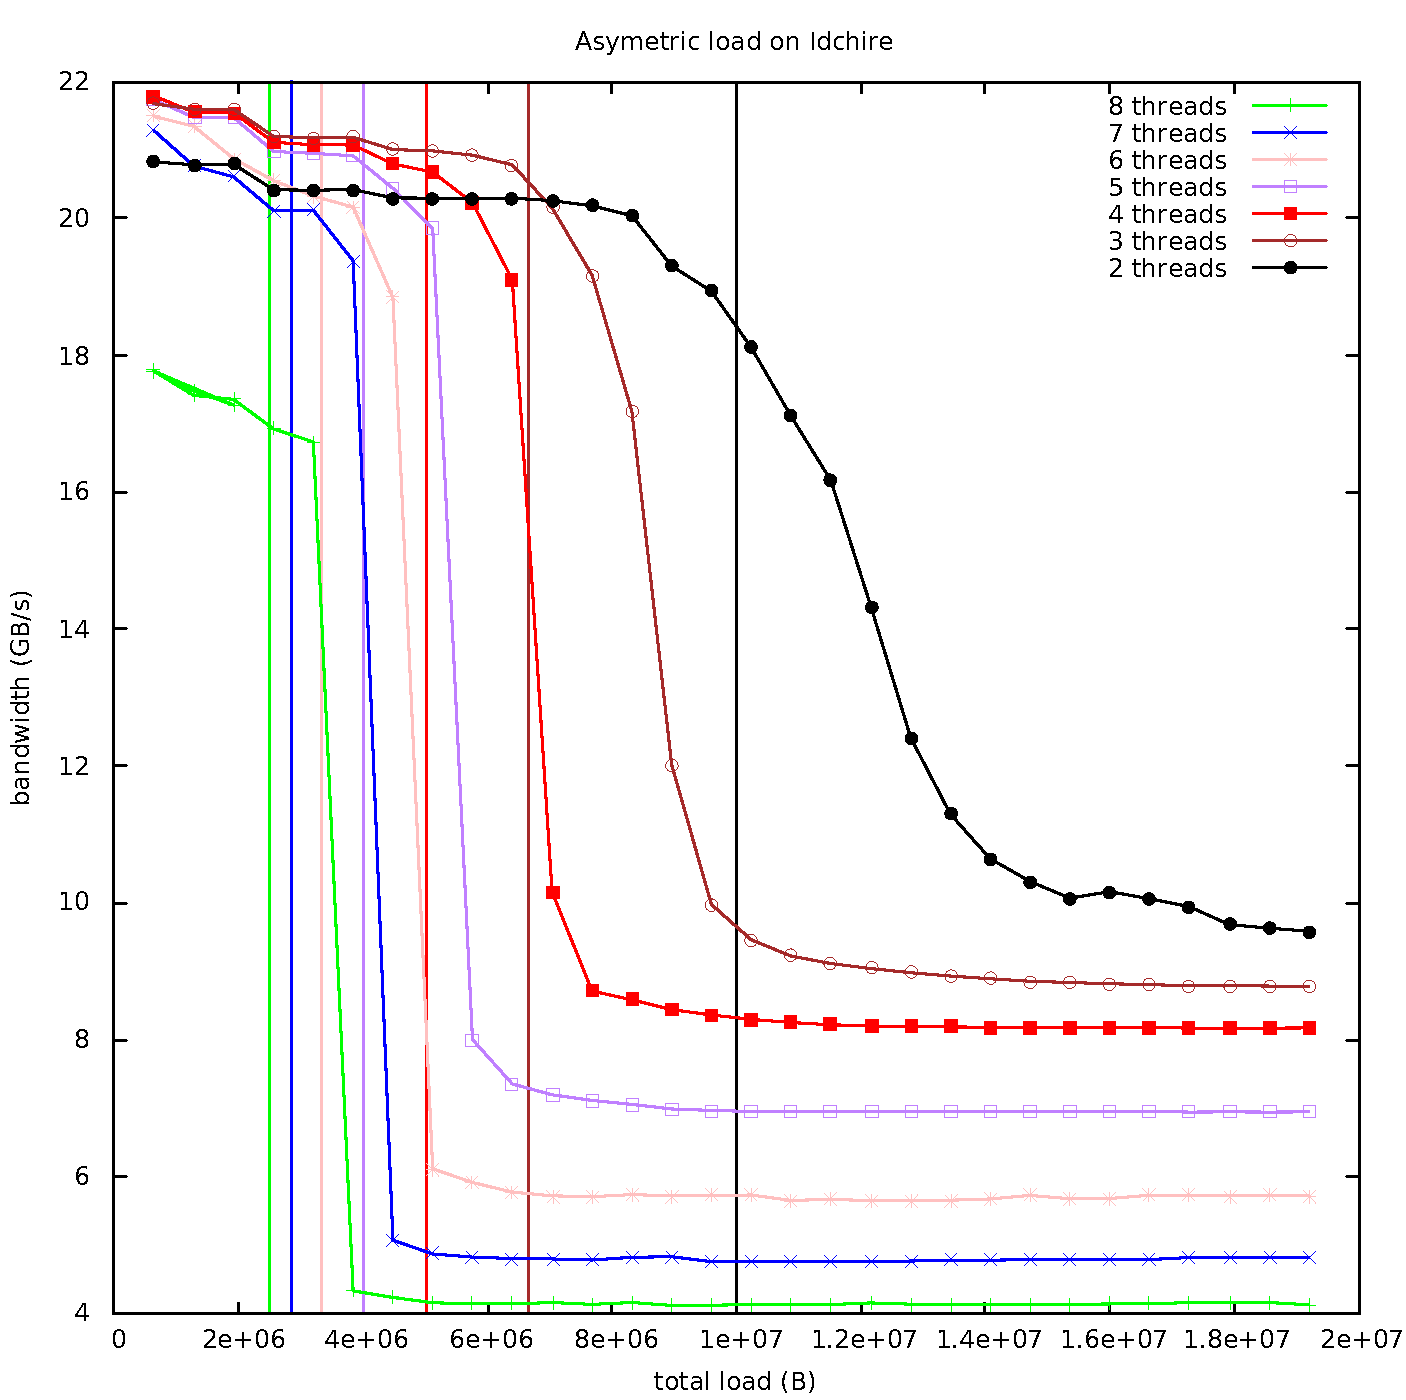
\includegraphics[width=\linewidth]{bw-asym-idchire.pdf}
  \label{fig:idchasbench}
\end{figure}
\begin{figure}[H]
  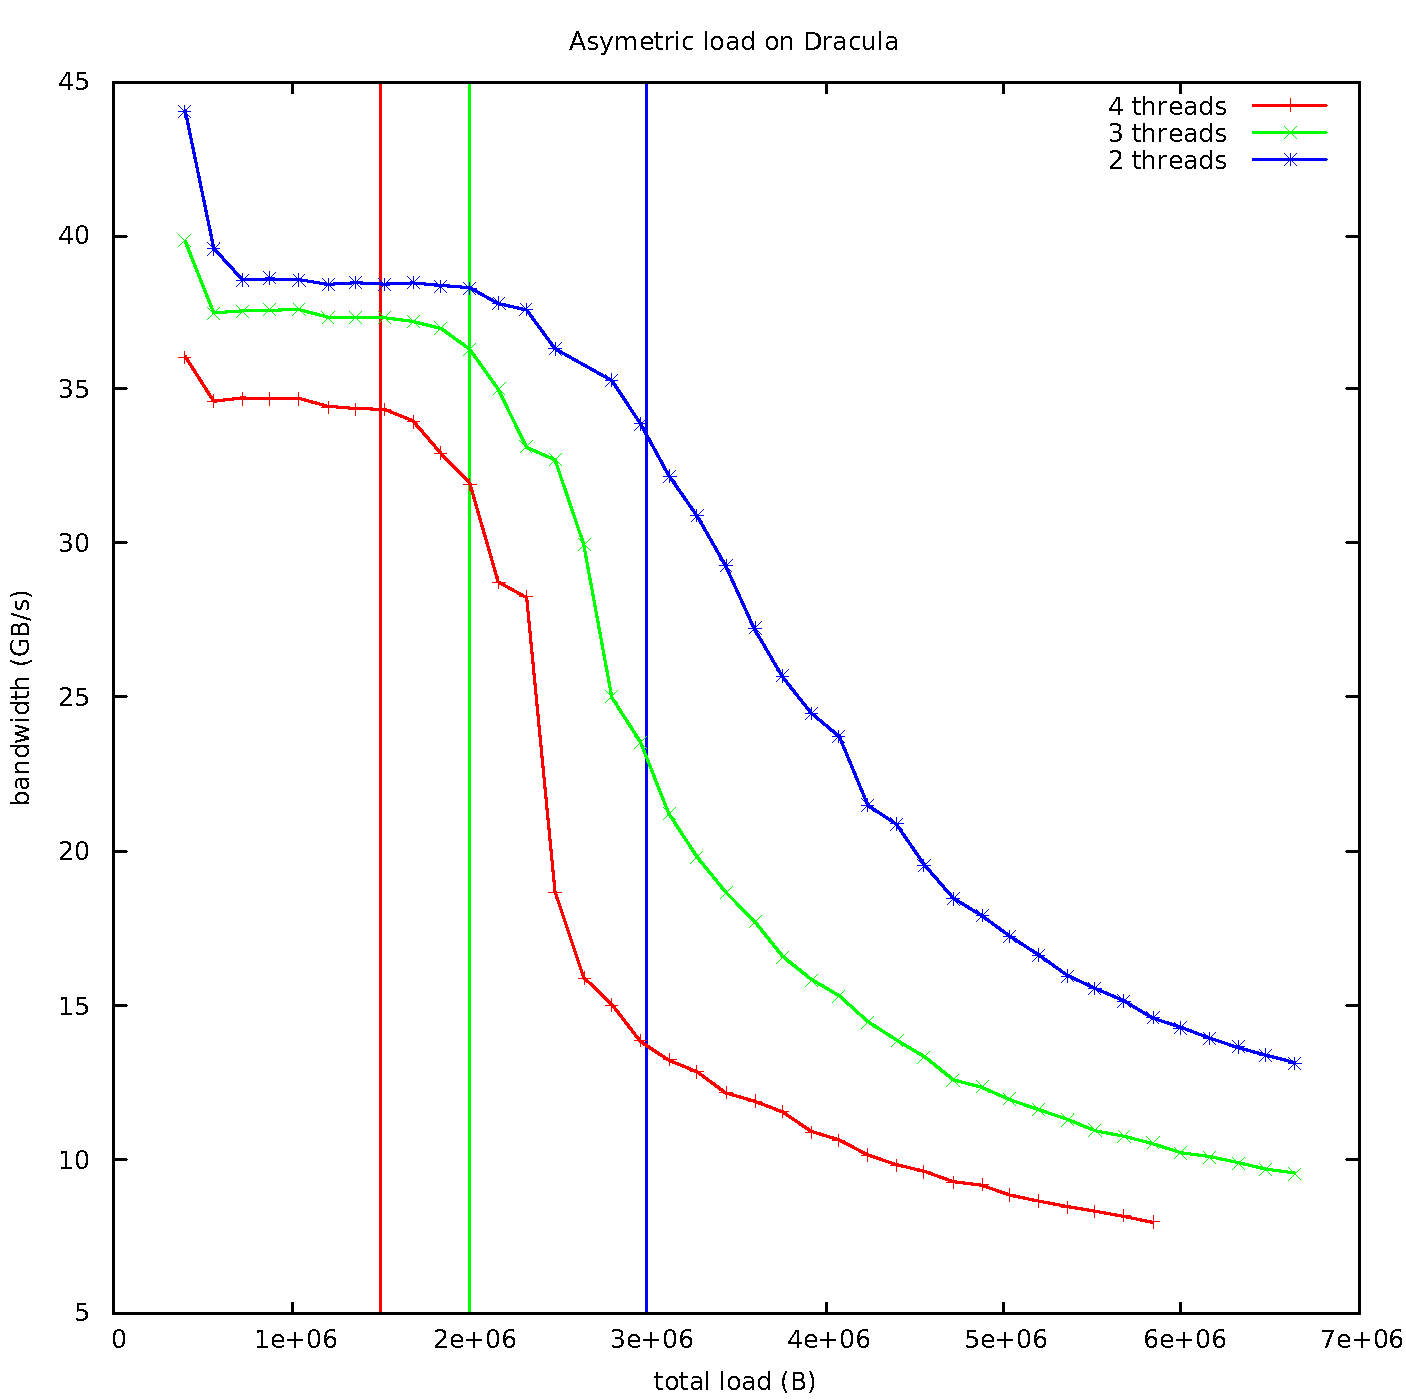
\includegraphics[width=\linewidth]{bench-asym-dracula.pdf}
  \label{fig:dracasbench}
\end{figure}
Nous avons ensuite essayé d'élargir le modèle en utilisant le même genre de principe. La
proposition suivante vient de mon tuteur :
\begin{th2}
Soit N un nombre de threads, $T_1, T_2, \cdots T_N$ les tailles des données auxquelles ces threads
accèdent respectivement, triées par ordre croissant. Soit C la taille du cache. On note $B_c$ la 
vitesse d'accès au cache et $B_m$ la vitesse d'accès à la mémoire principale. On affirme que :
$\forall i$, si $\sum_{j=1}^{i}{T_{j}} + \frac{B_m}{B_C} * T_i * (N - i) \leq C$, alors le
thread i ne subit pas de miss. Sinon, il est en full miss.
\end{th2}

Dans ce modèle, on va considérer que les threads sont soit en full miss, soit en full hits.
En fait, on considère que la zone de transition est suffisamment petite pour être ignorée.
\begin{proof}
  On reprend les notations de l'énoncé, ainsi que celles de la démonstrations précédente sur
  la distance de réutilisation.
  Posons i tel que le thread i soit en full hits, et le thread i+1 en full miss. Soit d une 
  donnée accédée par i. Exprimons $\Delta(d)$ en fonction de nos paramètres.
\\  $\forall j \leq i$, on a $\delta_j(d) = T_j$ comme précédemment.
 \\ $\forall k > i$, comme on a supposé que ces threads sont en full miss, et qu'on a posé
 $B_m$ comme la vitesse d'accès en mémoire, $\delta_k(d)=B_m * t$, où t est le temps qui 
 s'est déroulé entre deux accès successifs à d.
 On a donc $\Delta(d)= \sum_{j=1}^{i}{T_j} + \sum_{k=i+1}^{N}{B_m * t} = \sum_{j=1}^{i}{T_j}
 + B_m * t * (N - i)$
 \\Maintenant, comme on a supposé que i était en full hits, il accède à ses données à une
 vitesse $B_C$. Le temps de réaccéder à d est le temps qu'il met à accéder à toutes ses
 données (on est toujours sur un accès linéaire), c'est-à-dire que $t= \frac{T_i}{B_C}$.
 En réinjectant ce résultat dans la formule, on obtient :
 \\ $\Delta(d)=  \sum_{j=1}^{i}{T_j} + \frac{B_m}{B_C} * (N - i) * T_i $
 \\Et donc, si cette distance est inférieure à C, on a bien un thread en full hits dans
 une hypothèse LRU. On vérifie sans problème que cette formule est croissante selon i. 
 Donc en réalisant des essais successifs, on finit par distinguer les threads en full
 miss et les threads en full hits. 
\end{proof}
Ce modèle s'est révélé moins probant au moment de l'expérimentation. L'hypothèse 
que la zone de transition est négligeable est en fait trop forte : contrairement à
un cache en pur LRU qui afficherait une rupture nette de performance au moment où
les données dépassent la taille du cache (le programme passerait soudainement en 
full miss) les bandes-passantes mesurées prennent toutes les valeurs possibles entre la 
vitesse d'accès au cache et la vitesse d'accès à la mémoire principale. 
\\Dans l'idée d'obtenir un modèle plus précis, j'ai voulu m'intéresser plus aux algorithmes
de remplacement du cache.
\section{Algorithmes de remplacement}
Le problème principal ici est que les constructeurs ne donnent pas d'indications quant
à la politique qu'ils implémentent pour une architecture particulière. On en est 
réduit à faire des suppositions et à voir si les simulations correspondent aux
résultats expérimentaux. Il faudrait voir, en premier lieu, quels algorithmes pourrait
produire cette diminution continue de la bande-passante constatée empiriquement. On a déjà 
dit, en effet, qu'un cache purement LRU entrainerait un effondrement soudain du temps
d'accès, puisque dès l'instant où la taille des données dépasse la taille du cache, on 
ne fait plus que des miss.
\\Pour se donner une idée de la courbe qu'on peut attendre avec un cache, j'ai simulé
quelques politiques différentes. J'ai essayé notamment avec un algorithme extrêmement
naïf qui se contente de choisir une ligne à remplacer au hasard quand il doit rapatrier
une donnée. Cet algorithme a l'avantage de présenter cette courbe lisse qui semble 
s'approcher de la courbe rencontrée expérimentalement. Cela n'est cependant pas 
satisfaisant, car cette politique est trop naïve pour pouvoir être implémenté dans
la réalité. De plus, un cache qui se comporterait de cette manière n'exhiberait plus
cette ``protection'' des threads accédant à des données peu nombreuses qu'on a 
mise en évidence dans la partie précédente. En effet, dans cette configuration,
toutes les données sont traitées à la même enseigne.
\\On aurait pu imaginer un compromis entre une politique aléatoire et une politique
LRU. Ainsi, j'ai essayé de simuler un ``Not recently Used'', un algorithme qui choisit
la ligne victime aléatoirement parmi les lignes présentes en cache, exceptées celles 
qui ont été accédées relativement récemment. Cependant, cette politique, si elle 
permet de conserver la protection et la distinction entre les threads, exhibe une
discontinuité corrélée à la taille de la ``fenêtre de protection''. En clair, on
observe une chute brutale de la bande-passante quand les données dépassent la taille
du cache, ce saut augmentant avec la fenêtre. C'est en fait logique, puisqu'un tel
algorithme tend vers un simple LRU. 
\\J'ai également implémenté un algorithme Pseudo-LRU tel qu'il est décrit dans ce 
papier \cite{plru}. La LRU est ici approximée grâce à une structure en arbre. Chaque
noeud est marqué par un bit qui permet de savoir où le cache doit chercher la 
prochaine ligne à évicter. Quand le bit est à 0, le cache cherche dans l'arbre
gauche, sinon il va dans l'arbre droit. Ainsi dans l'exemple suivant, la ligne
marquée 2 sera la prochaine évictée.

\begin{tikzpicture}[->,>=stealth',level/.style={sibling distance = 5cm/#1,
  level distance = 1.5cm}] [label=tree1][H]
  \centering
\node [arn_w] {0}
    child{ node [arn_w] {1} 
            child{ node [arn_w] {0} 
							child{ node [arn_x] {12}}
							child{ node [arn_x] {15}}
            }
            child{ node [arn_w] {1}
							child{ node [arn_x] {18}}
							child{ node [arn_x] {2}}
            }                            
    }
    child{ node [arn_w] {0}
            child{ node [arn_w] {1} 
							child{ node [arn_x] {23}}
							child{ node [arn_x] {39}}
            }
            child{ node [arn_w] {0}
							child{ node [arn_x] {49}}
							child{ node [arn_x] {12}}
            }
		}
; 
\end{tikzpicture}

Lorsqu'on accède à une ligne - soit pour la remplacer, soit pour la lire ou y écrire -
on inverse tous les bits en remontant l'arbre. Ainsi, le remplacement de la ligne
marquée 2 par une ligne marquée 6 renverrait un arbre dans l'état suivant : 
\\\begin{tikzpicture}[->,>=stealth',level/.style={sibling distance = 5cm/#1,
  level distance = 1.5cm}] [label=tree2][h]
\node [arn_r] {1}
    child{ node [arn_r] {0} 
            child{ node [arn_w] {0} 
							child{ node [arn_x] {12}}
							child{ node [arn_x] {15}}
            }
            child{ node [arn_r] {0}
							child{ node [arn_x] {18}}
							child{ node [arn_x] {6}}
            }                            
    }
    child{ node [arn_w] {0}
            child{ node [arn_w] {1} 
							child{ node [arn_x] {23}}
							child{ node [arn_x] {39}}
            }
            child{ node [arn_w] {0}
							child{ node [arn_x] {49}}
							child{ node [arn_x] {12}}
            }
		}
; 

\end{tikzpicture}
On se convainc facilement que cet algorithme a pour effet de protéger la dernière 
donnée accédée. On peut imaginer des cas où ce n'est pas la donnée la plus ancienne
qui est évictée : il suffit pour cela que cette donnée soit situé dans la même partie
d'arbre que la donnée la plus récemment accédée. Néanmoins, cet algorithme semble
bien émuler un comportement LRU suffisamment efficacement pour l'usage courant.
\\J'ai voulu savoir si cette distinction pouvait expliquer l'écart de prévisions
avec le LRU pur. Il n'en est rien : dans le cas de accès très linéaires, cet 
algorithme se comporte très exactement comme un LRU. Il fallait donc chercher
autre chose. 
\\D'autres chercheurs ont essayé de reconstruire à partir de données empiriques
les algorithmes de remplacement de diverses architectures. C'est le cas du travail
présenté dans ce papier \cite{cachemodeling}. Décrire entièrement leur travail
dépasse la portée de ce rapport, mais l'idée générale est de s'arranger pour 
mettre le cache dans un état connu, puis de vérifier au bout de combien d'évictions
une ligne se trouve remplacé. On obtient pas ainsi d'informations sur la technique
d'implémentation du cache, mais le comportement se retrouve lui explicité. 
Malheureusement, les auteurs n'ont semblent-ils pas mis leur code en ligne, ce
qui m'a empêché de réaliser leurs tests sur mes architectures. Refaire leur 
travail à partir de leur description me semblait trop compliqué et je manquais de 
toute façon de temps. Néanmoins, les auteurs décrivent une politique de remplacement
qu'ils n'ont pu réussir à décrypter et qui semble produire des résultats très
similaires à ceux de mes architectures. Il s'agissait d'ailleurs d'architectures
Intel Core 2 E6750 et E8400, donc x86 comme les miennes. Il semble donc bien 
qu'Intel ait implémenté une stratégie plus complexes que ce qui est habituel sur
les architectures de ces dernières années.
\\Dans la mesure où les algorithmes de cache sont susceptibles de changer et qu'ils
sont parfois difficile à déterminer sur une architecture donnée, nous avons
voulu trouver un modèle qui ne reposerait pas sur une politique particulière.

\section{Modèle à base empirique}
Il serait donc intéressant de s'affranchir d'une politique de remplacement
particulière dans notre modèle. De la sorte, on pourrait espérer construire des prédictions
valables pour différentes architectures. L'idée serait de se baser sur une seule batterie
de tests pour en retirer les informations nécessaires à la construction d'un modèle plus
général. Dans notre cas, on aimerait se baser sur les résultats de bande-passante pour
obtenu pour un seul thread pour tenter ensuite de l'extrapoler pour des situations 
multithreadées et asymétriques. 
\subsection{construction du modèle}
Comment peut-on exploiter les données produites pour seulement un thread ? On va revenir
ici à l'idée de distance de réutilisation. L'hypothèse essentielle que l'on va faire 
pour ce modèle est que la probabilité de réaliser un miss sur une donnée est directement
fonction de cette distance de réutilisation, donc de la quantité de données qui a été
accédées et potentiellement rapatriée dans le cache. La vitesse d'accès est bien sûre
directement liée au taux de miss d'un thread. Dès lors, on va considérer que cette 
courbe représentant la vitesse de lecture en fonction de la taille des données d'un thread 
que l'on possède avec nos tests représente la vitesse d'accès en fonction de la distance
de réutilisation. C'est raisonnable dans la mesure où la distance de réutilisation
pour un thread est connue et exactement égale à la taille des données accédées par le
thread. Cela vient, encore une fois, de l'accès linéaire et cyclique que l'on fait sur
nos données. Reste maintenant à exprimer la distance de réutilisation de chacun des threads sur la 
base de cette hypothèse. Je l'ai exprimé récursivement de cette manière : 
\newtheorem{th3}{Théorème}
\begin{th3}
Soit N un nombre de threads, $T_1, T_2, \cdots T_N$ les tailles des données auxquelles ces threads
accèdent respectivement en ordre croissant. On note $\Delta(i)$ la distance de réutilisation globale 
d'une donnée accédée par le thread i,$\delta_i(j)$ la quantité de données accédées par un thread i
pendant l'intervalle entre deux accès à une même donnée du thread j, f la fonction empirique censée 
nous donner une vitesse d'accès en fonction d'une distance de réutilisation et $V_1, V_2 \cdots V_N$ 
les vitesses d'accès respectives de chacun des threads. On a, par définition de f, $\forall 
i, V_i = f(\Delta(i))$. Alors on dit que :
\\$\Delta(N)= \sum_{i=1}^{N}{T_{i}}$
\\Et pour un thread i quelconque, $\Delta(i)$ est solution de l'équation : 
\\$\Delta(i)= \sum_{j=1}^{i}{T_{j}} + \sum_{k=i+1}^{N}{V_k} * \frac{T_i} {f(\Delta(i))}$
\end{th3}
On peut donc grâce à ces formules déduire récursivement une vitesse d'accès pour chaque thread en
partant de la dernière. Voici le raisonnement :
\begin{proof}
  Le dernier thread étant nécessairement le plus lent et étant celui qui accède au plus de données,
  on est certain que toutes les données ont été accédées par tous les threads pendant l'intervalle
  de temps que lui a mis à accéder aux siennes. On a donc :
  \\$\Delta(N) = \sum{T_i}$
  \\Imaginons maintenant que l'on connaisse $\Delta(k)$ et donc $V_k$ pour k plus grand qu'un certain i.
  On va essayer d'exprimer chacun des $\delta_j(i)$. D'abord, pour $j \leq i$, on est sûr que 
  $\delta_j(i) = T_j$ puisque le thread j accède plus rapidement à moins de données que i. 
  \\Voyons maintenant pour $k > i$. On connait la vitesse d'accès $V_k$ de k, on a donc
  $\delta_k(i) = V_k * t_i $ où $t_i$ est l'intervalle de temps entre deux accès à une donnée de i.
  Or, ce temps s'exprime comme ceci : $t = \frac{T_i}{V_i} $.
  \\ Cette quantité est aussi égale à $\frac{T_i}{f(\Delta(i))}$ par définition de f.
  \\Finalement, on obtient : 
  $\delta_k(i) = V_k * \frac{T_i}{f(\Delta(i))}$
\\ Et en réinjectant ceci dans l'expression de $\Delta(i)$, on trouve : 
\\  $\Delta(i) = \sum_{j=1}^{N}{\delta_j(i)} = \sum_{j=1}^{i}{T_j} + \sum_{k=i+1}^{N}{V_k} * \frac{T_i}{f(\Delta(i))}$
\end{proof}

Les équations étant basées sur une fonction empirique, elles ne sont pas résolvables analytiquement, 
mais on peut par contre utiliser une méthode numérique pour trouver une solution approchée. J'ai 
choisi d'utiliser une méthode de Newton, épaulée au besoin (quand on n'est pas capable de fournir 
une valeur initiale de la solution) par une simple bisection. Pour cela, j'ai utilisé la 
bibliothèque numpy de python. 
\begin{lstlisting}[language=python]
#take a reverse sorted thread sizes list and 
#returns the list of corresponding bandwidths
def calculate_cache(lThreads, lBw, data):
#empirical continuous function from discrete datas
    f = fromdata(data)
    #if no more threads to treat, returns
    if ( not lThreads):
        return lBw
    #first and biggest datas
    elif (not lBw):
        bw = f(sum(lThreads))
        lBw.append(bw)
        lThreads.pop(0)
        return calculate_cache(lThreads, lBw, data)
    else:
        try:
            thrsum = sum(lThreads)
            lBwsum = sum(lBw)
            def func(x):
                return (f(x) * (x - thrsum) - (sum(lBw))*lThreads[0])
            xopt = scipy.optimize.newton_krylov(func, thrsum, f_tol = 1.0)
            lBw.append(f(xopt))
            lThreads.pop(0)
            return calculate_cache(lThreads, lBw, data)
        except ValueError:
            # newton approximation can fail when bw is too big
            # in this case we try to approach a solution
            # by a bisection method
            def func(x):
                return (f(x) * (x - thrsum) - (sum(lBw))*lThreads[0])
            xopt = bisect(func, lThreads[0], 2 * thrsum, 0)
            lBw.append(f(xopt))
            #bw = lBw[-1]
            #lBw.append(bw)
            lThreads.pop(0)
            return calculate_cache(lThreads, lBw, data)

\end{lstlisting}
Le code complet est trouvable en annexe. Voilà à quel point j'en étais à la fin de mon stage.
Comme on va le voir, ce modèle souffre encore de grosses approximations qu'il aurait été intéressant
d'essayer de résoudre.
\subsection{limitations}
Malheureusement, il m'a manqué du temps pour tester ce modèle extensivement. Il semble qu'il soit encore
trop approximatif dans les cas critiques où la somme des données des threads s'approchent de la taille 
du cache, et il est généralement trop optimiste. Remarquons tout de même qu'on retrouve les résultats
de protection des threads chargeant peu de données, qui se retrouvent en full hits. Si l'on manque 
encore de recul pour l'analyse, des failles peuvent clairement être mises en avant.
\\La principale est que ce modèle tient la vitesse d'accès à la mémoire pour une constante, alors que 
l'on a déjà vu dans la section \ref{subsec:ressources} que cette vitesse est dépendante du nombre 
de threads qui tentent d'y accéder. 
\\Ce modèle est donc conduit à surestimer la vitesse que peut espérer atteindre un thread qui doit
ramener toutes ses données depuis la mémoire principale. Cela peut en partie expliquer la tendance
à surestimer les valeurs des vitesses de notre modèle.
\\J'ai cherché à améliorer la situation en utilisant également comme base les résultats empiriques
provenant de plusieurs threads réalisant un travail symétrique. Les valeurs des vitesses d'accès à
la mémoire principale étaient au moins correctes si l'on arrivait à deviner combien de threads 
allaient se trouver en full miss. L'idée était de faire tourner plusieurs fois l'algorithme avec 
les différentes données expérimentales jusqu'à trouver la prédiction la plus cohérente. Je vérifiais
la cohérence de la manière suivante : quand j'utilisais par exemple les données générées avec
trois threads, je vérifiais que l'on avait bien prédit que trois threads se retrouvaient en situation
de full miss. Sinon, je recommençais avec une autre valeur. 
\\Cette méthode ne semblait pas donner de bien meilleurs résultats. Il reste, il me semble, un problème
fondamentale à ce modèle qui est le suivant : comment déterminer le partage de la bande-passante 
depuis la mémoire principale quand certains threads font partiellement des miss et partiellement 
des hits. Au point où j'en suis, il me semble qu'un modèle plus pointu devra apporter une réponse
à ces questions.

\chapter{Conclusion}
J'ai donc présenté dans ce rapport l'ensemble de mes activités durant mes six mois de stage à l'Inria
Grenoble. Sur un plan professionnel, je crois avoir réussi à faire profiter mon équipe de mes compétences,
notamment grâce au travail réalisé sur le benchmark qui a été réutilisé par d'autres membres dans le cadre
d'un travail annexe. Je trouve dommage de n'avoir pas pu aboutir sur le sujet de la prédiction de cache. 
Il me semble néanmoins avoir exploré des pistes intéressantes, qui peuvent former une bonne
base de réflexion à de futurs travaux.
\\Sur un plan plus personnel, ces six mois m'ont permis de développer très largement mes connaissances et
mes compétences. J'ai désormais une compréhension beaucoup plus pointue des sujets traitants notamment
d'architectures bas niveau, de modèles mémoire, des problématiques de compilation ou des supports 
d'exécution. J'ai aussi pu prendre de l'expérience en développement dans différents langages,
essentiellement le python et le C++ ainsi que en ocaml. Plus que cela, j'ai pu découvrir le monde de la
recherche et son fonctionnement, une expérience qui, je l'espère, me sera utile dans mon parcours 
professionnel, et qui devrait être mise à profit très rapidement puisque je reviendrai travailler dans
le laboratoire d'ici un mois, temporairement en tant qu'ingénieur. J'espère à l'avenir avoir l'occasion
de pousser le processus de recherche jusqu'au bout et notamment jusqu'à la rédaction d'un article, ce
que je n'ai pas eu l'occasion de faire ici. Ceci conclut donc ce rapport et mon stage de fin d'études.
\bibliographystyle{plain} 
\bibliography{report}
\begin{appendices}
  \chapter{Annexes}
  \section{fonction main du benchmark de load, avec allocations et répartitions des threads}
  \begin{lstlisting}

int main(int argc, char ** argv)
{
	double * tab;
	pthread_t * thrTab;
	pthread_barrier_t bar;


	int quantum;
	int BytesPerWord;
	long nb_iter;
	unsigned long load_bytes;
#ifdef USE_PADDING
// We introduce some padding in data to see if 
// something is changed
	int var_padding = (1 << 25);
#endif


	//Parsing args and initializing param
	//in order to get number of threads,
	//slow threads, places, etc.
	int ret = parseArg(argc, argv,  &param);
	if (ret < 0)
	{
		printf("usage : ./load -n=<threads number> -slow=<number of slow threads> -size=<power of two> -ratio=<ratio slow size / fast size> -places=<core places| close | spread>\n");
		exit(EXIT_FAILURE);
	}
	if (param == NULL)
	{
		cout << "param not allocated !!" << endl;
		exit(EXIT_FAILURE);
	}

	param->info();
	


	printf(HLINE);
	BytesPerWord = sizeof(double);
	printf("This system uses %d bytes per DOUBLE PRECISION word.\n",
			BytesPerWord);

	printf(HLINE);

	if  ( (quantum = checktick()) >= 1) 
		printf("Your clock granularity/precision appears to be "
				"%d microseconds.\n", quantum);
	else
		printf("Your clock granularity appears to be "
				"less than one microsecond.\n");
	
	
	//pinning main thread on cpu 0 (on a numa architecture, data could 
	// be allocated on another node otherwise)
	cpu_set_t sets;
	CPU_ZERO(&sets);
	CPU_SET(0, &sets);
	int s = pthread_setaffinity_np(pthread_self(),sizeof(cpu_set_t), &sets);
	if (s != 0)
	{
		printf("could not set affinity\n");
		exit(EXIT_FAILURE);
	}
	
	


	int nbFst = param->nbThread - param->nbSlow;
	//initializing tab containing data to be loaded
#if defined(__gnu_linux__) && defined(USE_HUGE) 
	//using mmap for allocating hugepages
	void * ptrvoid = mmap(NULL, (param->globsiz + 8) * sizeof(double), PROT_READ | PROT_WRITE, MAP_PRIVATE | MAP_ANONYMOUS | MAP_HUGETLB | HUGE_MAP , -1, 0 );
	if (ptrvoid == MAP_FAILED)
	{
		cout << "could not allocate tab with mmap" << endl;
		exit(EXIT_FAILURE);
	}
	tab = (double *) ptrvoid;

#else
#ifdef USE_PADDING
	//padding
	tab = new double[param->globsiz + 8 + param->nbThread * var_padding];
#else//USE_PADDING
	tab = new double[param->globsiz + 8 ];
#endif//USE_PADDING
#endif //HUGE
	if(tab == NULL)
	{
		cout << "could not allocate tab" << endl;
		exit(EXIT_FAILURE);
	}
	//storing old value for freeing
	double * oldtab = tab;
	//aligning on 32 bytes for intrinsics and
	//assembly constraint
	tab = (double *)align_ptr((char *)tab, 32);
#pragma omp for
	for (size_t i = 0; i <  param->globsiz; i++)
	{
		tab[i]= 3.4;
	}

	printf(HLINE);
	print_status();
	printf(HLINE);
	

	// getting number of iterations, we want to do approximately 2^25 cycles

	long * iter = NULL;
	load_bytes = 0;
	if (param->thrSizes != NULL)
	{
		iter = get_tab_iter(param->thrSizes, param->nbThread);
		nb_iter = 0;
		for (int i = 0; i < param->nbThread; i++)
		{
			//nb_iter += iter[i] ;
			load_bytes += iter[i] * param->thrSizes[i] * sizeof(double); 
		}
		nb_iter = array_sum(iter, param->nbThread);
}
	else
	{
		nb_iter = get_nb_iter(param->globsiz);
		load_bytes = nb_iter * param->globsiz;
	}


	long bytes = param->globsiz * sizeof(double);
	printf(HLINE);
	printf("N = %ld, %d threads will be called, loading %d%c bytes of data \n", param->globsiz, param->nbThread, siz(bytes), units(bytes));
	printf(HLINE);



	// array that will contain pthread identifiers
	thrTab = (pthread_t *)malloc(param->nbThread * sizeof(pthread_t));
	
	*thrTab= pthread_self();
	// we don't want threads to start loading before having been
	// pinned, so we put a barrier
	pthread_barrier_init(&bar, NULL, param->nbThread);
	args_t hargs[param->nbThread];

	//array for timestamp (in order to get global throughput
	// at the end)
	double *times = new double[param->nbThread];
	unsigned long *cycles = new unsigned long[param->nbThread];
	


	if (param->thrSizes == NULL)
	{


		int i;
		// this offset will be incremented by the size
		// of the array we want our thread to work on
		intptr_t offset = 0;
		if (param->nbSlow == param->nbThread)
			offset += param->ssiz;
		else
			offset += param->fsiz;

		for(i = 1; i < nbFst; i++)
		{
			//address of data start for this thread
#ifdef USE_PADDING
			hargs[i].t = tab + offset + var_padding;
#else//USE_PADDING
			hargs[i].t = tab + offset ;
#endif//USE_PADDING
			hargs[i].bar = &bar; 
			hargs[i].size = param->fsiz; 
			hargs[i].niter = nb_iter; 
			hargs[i].time = times + i; 
			hargs[i].cycle = cycles + i; 
			pthread_create(thrTab + (intptr_t)i, NULL, handler, (void *) &hargs[i]);
			offset +=  param->fsiz;
		}

		for(; i < param->nbThread; i++)
		{
			hargs[i].t = tab + offset;
			hargs[i].bar = &bar; 
			hargs[i].size = param->ssiz; 
			hargs[i].niter = nb_iter; 
			hargs[i].time = times + i; 
			hargs[i].cycle = cycles + i; 
			pthread_create(thrTab + (intptr_t)i, NULL, handler_slw, (void *) &hargs[i]);
			offset +=  param->ssiz;
		}

	}
	// thrSizes is set
	// user has entered data sizes
	else
	{
		intptr_t offset = param->thrSizes[0];
		int i;
		for( i = 1; i < nbFst; i++)
		{
			//padding with adding_var doubles
			hargs[i].t = tab + offset ;
			hargs[i].bar = &bar; 
			hargs[i].size = param->thrSizes[i]; 
			//hargs[i].niter = nb_iter; 
			hargs[i].niter = iter[i]; 
			hargs[i].time = times + i; 
			hargs[i].cycle = cycles + i; 
			pthread_create(thrTab + (intptr_t)i, NULL, handler, (void *) &hargs[i]);
			offset +=  param->thrSizes[i];
		}
		for(; i < param->nbThread; i++)
		{
			//padding with adding_var doubles
			hargs[i].t = tab + offset ;
			hargs[i].bar = &bar; 
			hargs[i].size = param->thrSizes[i]; 
			//hargs[i].niter = nb_iter; 
			hargs[i].niter = iter[i]; 
			hargs[i].time = times + i; 
			hargs[i].cycle = cycles + i; 
			pthread_create(thrTab + (intptr_t)i, NULL, handler_slw, (void *) &hargs[i]);
			offset +=  param->thrSizes[i];
		}
	}



	//Placing threads on appropriate cpu
	//If either fstThrList or slwThrList
	//is set to null, then it means that 
	//all threads are either fast or slow
	if (param->fstThrList != NULL)
	{
		int s;
		cpu_set_t sets[nbFst];
		for (int k = 0; k < nbFst; k++)
		{
			CPU_ZERO(&sets[k]);
			CPU_SET(param->fstThrList[k], &sets[k]);
			printf("fast thread [%d] pinned on cpu %d\n", k, param->fstThrList[k]);
			s = pthread_setaffinity_np(thrTab[k],sizeof(cpu_set_t), &sets[k]);
			if (s != 0)
			{
				printf("could not set affinity\n");
				exit(EXIT_FAILURE);
			}
		}
		
	}

	if (param->slwThrList != NULL)
	{
		int s;
		cpu_set_t sets[param->nbSlow];
		for (int k = 0; k < param->nbSlow; k++)
		{
			CPU_ZERO(&sets[k]);
			CPU_SET(param->slwThrList[k], &sets[k]);
			s = pthread_setaffinity_np(thrTab[nbFst + k],sizeof(cpu_set_t), &sets[k]);
			if (s != 0)
			{
				printf("could not set affinity\n");
				exit(EXIT_FAILURE);
			}
			printf("Slow thread [%d] pinned on cpu %d\n", k, param->slwThrList[k]);
		}

	}


	// launching main thread
	// slow threads if there is 
	// no fast thread
	// fast thread otherwise
	hargs[0].t = tab ;
	hargs[0].bar = &bar; 
	//hargs[0].niter = nb_iter; 
	if (iter != NULL)
		hargs[0].niter = iter[0]; 
	else
		hargs[0].niter = nb_iter; 
	hargs[0].time = times ; 
	hargs[0].cycle = cycles; 
	if (param->thrSizes == NULL)
	{
		if(param->nbThread == param->nbSlow)
		{
			hargs[0].size = param->ssiz; 
			handler_slw((void *)&hargs[0]);
		}
		else
		{
			hargs[0].size = param->fsiz; 
			handler((void *)&hargs[0]);
		}
	}
	//case user had entered thread sizes as inputs
	else
	{
		hargs[0].size = param->thrSizes[0];
		if(param->nbThread == param->nbSlow)
			handler_slw((void *)&hargs[0]);
		else
			handler((void *)&hargs[0]);
			

	}


	for (int k = 0; k < param->nbThread; k++)
		pthread_join(thrTab[k], NULL);
	
	double maxtime = *(std::max_element(times, times + param->nbThread));
	unsigned long maxcycle = *(std::max_element(cycles, cycles + param->nbThread));

	//double ld = sizeof(double) * param->globsiz * nb_iter ;
	printf("Global throughput : %f %cB/s\n", siz_d(load_bytes / maxtime), units_d(load_bytes / maxtime));
	printf("Global bytes per cycle : %f %cB/c\n", siz_d(load_bytes / maxcycle), units_d(load_bytes / maxcycle));
	printf("Estimated frequency : %f %cHz\n", siz_d(maxcycle / maxtime), units_d(maxcycle / maxtime));

	//free param
	delete[] times;
	delete[] cycles;
	free(thrTab);
#if defined(__gnu_linux__) && defined(USE_HUGE) 
	munmap((void *)oldtab, ((param->globsiz + 8) * sizeof(double) ));
	//munmap((void *)oldtab, std::min((size_t)(1 << 27), ((param->globsiz + 8) * sizeof(double))));
#else
	free(oldtab);
#endif
	delete param;
	return 0;
}
  \end{lstlisting}
  \section{programme Ocaml de simulation d'accès cache}
\begin{lstlisting}[language=caml]
open Array
open Printf

module type Cache = sig
  type  t
  val initSimpleTree : int ->  t
  val insertVal : int -> float ->  t ->  t   
  val getValAtCache : int ->  t ->  t * float option
end

  (*Look for a variable, first in cache, then in memory in case of miss
   * insert new value in cache in case of miss
   * returns a boolean, the searched value and the new cache
   * The boolean is true in case of hit, false in case of miss
   * *)
let getValAt addr tree arr = 
  let newTree, res = PLRU.getValAtCache addr tree  in  match  res with
    | None -> false, arr.(addr), PLRU.insertVal addr arr.(addr) newTree
    | Some v -> true, v, newTree

    (*loop and emulate load niter times
     * *)
let rec loop niter arr = 
  let rec inter it arr cache acc = 
  if (it < niter) then 
    ((* let plru = (module PLRU : Cache) in *)
      let hit, res, newCache = getValAt (it mod (Array.length arr)) cache arr  in 
      if (hit) then 
        inter (it + 1) arr newCache (acc + 1)
      else
        inter (it + 1) arr newCache acc 
    )
  else
    acc
  in
  let cache = PLRU.initSimpleTree 5 in
  inter 0 arr cache 0;;


let () = 
  Random.self_init ();
  let arrlen = if (Array.length Sys.argv > 1) then int_of_string (Sys.argv.(1)) else 100 in
  let  memArray = Array.make arrlen 0.0 in
    for i = 0 to (Array.length memArray - 1) do memArray.(i) <- (float_of_int i) done;
  (*let cache = PLRU.initSimpleTree 5 in*)
  printf "%d hits \n" (loop 10000 memArray ) 





\end{lstlisting}
\section{Programme Ocaml de simulation de PLRU }
\begin{lstlisting}[language=caml]

type  'a t = Node of bool *  'a t *  'a t | Leaf of (int * 'a) option 


  (* simple balanced binary tree *)
  (*
let rec initSimpleTree hght = 
  if (hght == 0) then Leaf None else Node(true, initSimpleTree (hght - 1), initSimpleTree (hght - 1))
  *)

let rec initSimpleTree hght = 
  if (hght == 0) then Leaf None else 
    ( if (hght mod 2 == 0 ) then  Node(true, initSimpleTree (hght - 1), initSimpleTree (hght - 1))
    else Node(false, initSimpleTree (hght - 1), initSimpleTree (hght - 1))
    )

(*search for a value in cache, return Some if success, None if fail*)
let rec getValAtCache addr t = match t with
  | Node(b, left, right) -> 
      (let treeLeft, resLeft = getValAtCache addr left and treeRight, resRight= getValAtCache addr right in
      match (resLeft, resRight) with 
    | Some a, _ -> Node(false, treeLeft, treeRight), Some a 
    | None, Some b -> Node(true, treeLeft, treeRight), Some b
    | None, None -> Node(b, treeLeft, treeRight), None
    )
  | Leaf(Some(a, v)) when (a == addr) -> t, Some v
  | Leaf _ -> t, None

  (*insert val in cache in case of miss*)
let rec insertVal addr v tree =  match tree with
  | Leaf(_) -> Leaf(Some(addr, v))
  | Node(true, ltree, rtree) ->  Node(false, insertVal addr v ltree, rtree )
  | Node(false, ltree, rtree) ->  Node(true,  ltree, insertVal addr v rtree )
\end{lstlisting}
  script python d'estimation des vitesses d'accès.
\begin{lstlisting}[language=python]
#!/usr/bin/env python3
import scipy.optimize
import numpy
import re
import sys
from random import randint

#input_name = "data-dracula.txt"
# datas from dracula benchmarks
input_name = "results1.txt"
input_name2 = "results2.txt"
input_name3 = "results3.txt"
input_name4 = "results4.txt"

class NoArgException(Exception):
    pass

# get a continuous and differentiable function
# from a data set
# not used in the code
def femp_interpol(datak, datav):
    coeff = numpy.polyfit(datak, datav, len(datak) - 1)
    diccoeff = [(i, coeff[len(datak) - i - 1]) for i in range(len(coeff))]
    def inter(x):
        return sum([ pow(x, i) * v for (i, v) in diccoeff])
    return inter

# this function takes a float and a sets of data
# approximate the value for input x by simply linking points
def femp(x, data):
    xint = int(x)
    sorted_keys = sorted(data.keys())
    fkey  = sorted_keys[0]
    skey  =  sorted_keys[1]
    lkey = sorted_keys[-1]
    if (xint < fkey):
        return data[fkey]
    if(xint > lkey):
        return data[lkey]
    #print("keys : {} {}\n".format(fkey , skey))
    # difference between two consecutives points
    delta = skey - fkey
    base = fkey
    x_rounded = (((xint - base) // delta ) * delta) + base
    lbda = (x - x_rounded ) / float(delta)
    bwx = (1 - lbda) * data[x_rounded] + lbda * data[x_rounded + delta]
    return bwx

# approximate a zero with a bisection
# less efficient than newton, used as a plan B
def bisect(f, x1, x2, n):
    if (( abs(x1 - x2) < 0.0001) or ( n > 10000) or (abs(f(x1)) < 0.001)):
        return x1
    if( f(x1) * f(x2) < 0 ):
        y3 = f( (x1 + x2) / 2)
        if (y3 * f(x1) < 0):
            return bisect(f, x1, (x1 + x2) / 2, n + 1)
        else:
            return bisect(f, (x1 + x2) / 2, x2, n + 1)
    else:
        #case initial points happen to be of same sign
        if (randint(0, 100) < 50) :
            return bisect(f,x1 + x2, 2 * x2, n + 1)
        else:
            return bisect(f,x1 / 2, x2  / 2, n + 1)

# ask user for thread sizes input
# can be passed in standard input (supports EOF
# for terminating
def get_threads():
    tab=[]
    print("Enter data size for each threads, press <Return> when finished")
    s = sys.stdin.readline()
    while(s and (not re.match('^$', s))):
        s = s.strip()
        try:
            tab.append(int(s))
        except ValueError:
            print("Enter number")
        s = sys.stdin.readline()
            
    print(tab)
    return tab




#get a function femp based on data passed as parameters
def fromdata(test):
    return lambda x: femp(x, test)

# returns the derivative of the function passed as parameters
# 
def derivate(f, delta):
    def func(x0) :  
         return ((f(x0 + delta) - f(x0)) / float(delta))
    return  func

#take a reverse sorted thread sizes list and 
#returns the list of corresponding bandwidths
def calculate_cache(lThreads, lBw, data):
    f = fromdata(data)
    if ( not lThreads):
        return lBw
    elif (not lBw):
        bw = f(sum(lThreads))
        lBw.append(bw)
        lThreads.pop(0)
        return calculate_cache(lThreads, lBw, data)
    else:
        try:
            thrsum = sum(lThreads)
            lBwsum = sum(lBw)
            def func(x):
                return (f(x) * (x - thrsum) - (sum(lBw))*lThreads[0])
            xopt = scipy.optimize.newton_krylov(func, thrsum, f_tol = 1.0)
            lBw.append(f(xopt))
            lThreads.pop(0)
            return calculate_cache(lThreads, lBw, data)
        except ValueError:
            # newton approximation can fail when bw is too big
            # in this case we try to approach a solution
            # by a bisection method
            def func(x):
                return (f(x) * (x - thrsum) - (sum(lBw))*lThreads[0])
            xopt = bisect(func, lThreads[0], 2 * thrsum, 0)
            lBw.append(f(xopt))
            #bw = lBw[-1]
            #lBw.append(bw)
            lThreads.pop(0)
            return calculate_cache(lThreads, lBw, data)



try:
    datafile = sys.argv[1]
except:
    raise NoArgException("you must give a data file as input")

with open(datafile, "r") as dataf:
    line = dataf.readline()
    datakeys = []
    dataval = []
    data = dict()
    # retrieve data from files
    while(line ):
        l = line.split()
        data[int(l[0])]= float(l[1])
        datakeys.append(int(l[0]))
        dataval.append(float(l[1]))
        line = dataf.readline()


thrlist = get_threads()
# we want to iterate on threads in
# decreasing order 
tabThr = sorted(thrlist, reverse=True)
lBw = calculate_cache(tabThr, [], data)
\end{lstlisting}
\end{appendices}
\end{document}
